\documentclass[11pt,a4paper]{book}
\usepackage{Appunti_universitari}

\begin{document}
\title{Interazione uomo macchina}
\author{Jacopo De Angelis}
\maketitle

\pagebreak
\tableofcontents
\pagebreak

\chapter{Modulo 1: Concetti di base}
\section{Cos'è l'interazione uomo macchina?}
\begin{center}
Definizione standard 

\textit{"HCI (Human-Computer Interaction) è una disciplina che si occupa della progettazione, realizzazione e valutazione di sistemi interattivi con capacità computazionali destinati all'uso umano e dello studio dei principali fenomeni che li circondano"} - \textit{Associacion for Computing Machinery}
\end{center}

L'usabilità di un sistema è spesso trascurata all'interno dell'ambito lavorativo italiano, non per faciloneria ma perchè le risorse da adibire a questo ambito sono una spesa che non viene vista come essenziale nella produzione del valore per andare avanti. 

Il problema viene aggravato dall'outsourcing verso paesi dove il costo del lavoro sia inferiore e, ultimamente, anche da sistemi di ML che sono in grado, con grado di precisione sempre maggiore grazie al deep learning, di sviluppare codice funzionante. Ma cosa viene assegnato ai lavoratori esterni? Ciò che è altamente formalizzato, in modo da lasciare poche possibilità di variazione dalle richieste dei clienti.

Cosa rimane difficile da esternalizzare? Il contatto del cliente, sia durante la prima raccolta di requisiti funzionali, sia le successive interazioni con esso per cambiamenti incrementativi, variazioni di funzionalità o feedback.

L'usabilità è quella caratteristica che rende "facile la vita" al cliente.

\noindent\rule{\textwidth}{1pt}
\begin{center}
\textit{Piccola digressione}
\end{center}
\textbf{Perchè la concorrenza moderna rende sempre più importante l'analisi dell'interazione uomo macchina?}

In un contesto monopolistico le aziende non sono invogliate a produrre la soluzione "migliore"\footnote{Dove per migliore si intende quella che prende in considerazione più metriche come usabilità, efficienza, efficacia, design, ecc} ma solo quella più efficiente a livello di costo marginale.   

Cosa vuole dire questo? Che nella moderna concorrenza derivante da sistemi di sviluppo sempre più semplici e un'offerta più rapida tramite internet, per ottenere quote di mercato le aziende devono iniziare a pensare non solo al "funziona?" ma anche al "come lo faccio funzionare?"
\\\noindent\rule{\textwidth}{1pt}

\textbf{"Qui non si impara a fare delle interfacce usabili, si impara a riconoscere l'usabilità delle interfacce"} ovvero impariamo strumenti che ci possono portare a fare delle belle interfacce, certo, ma soprattutto ci permette di riconoscere cosa renda \underline{buona} un'interfaccia.

La disciplina nasce negli anni '80 ma l'interazione con le macchine (intese come calcolatori) esiste dagli anni'40, semplicemente prima l'utente era ultra specializzato mentre ora quasi tutti possono accedere ad un PC e con questo interagire tramite un'interfaccia.

Dal 1983 si tiene la conferenza annuale \href{https://dl.acm.org/conference/chi}{ACM CHI}. In questi casi tre aree disciplinari si incontrano:
\begin{itemize}
	\item ergonomia
	\item informatica
	\item psicologia comportamentista
\end{itemize}
\begin{figure}[h!]
	\begin{center}
		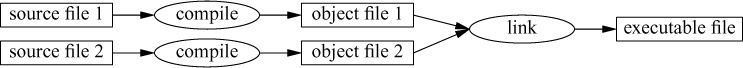
\includegraphics[scale=0.6]{img/001.jpg}
		\caption{HCI e le sue componenti}
		\label{fig: 001}
	\end{center}
\end{figure}
Dobbiamo ricordare sempre una cosa: dobbiamo lasciarci alle spalle l'utente ideale, l'utente senza faccia e senza capacità, e iniziare a pensare all'utente reale, ovvero a chi, idealmente, è diretta la nostra interfaccia. \underline{L'utente non siamo noi}. Proprio per questo le interviste, i test con esterni, i mockup sono utili, perchè ci permettono di vedere la nostra idea attraverso gli occhi di altri. Esempio banale: la nostra interfaccia basata sul colore potrebbe essere altamente confusionaria per un daltonico. Un'applicazione mobile dove tutti i comandi sono sulla destra potrebbe essere difficile da usare per un mancino.

\textbf{Ergonomia cognitiva}: studio dell'interazione tra l'uomo e gli strumenti per l'elaborazione di informazioni studiando i processi cognitivi coinvolti (percezione, attenzione, memoria, pensiero, linguaggio, emozioni) e suggerendo delle soluzioni per migliorare tali strumenti.

\section{Perchè è difficile progettare perchè l'interazione sia "buona"?}
Ci sono tre ragioni, idealmente:
\begin{enumerate}
	\item \textbf{La varietà dei sistemi interattivi}: cellulari, computer, cloche, macchine da cucina, tablet...
	\item \textbf{La varietà degli utenti}: fasce d'età, background culturale, condizioni mediche...
	\item \textbf{La varietà degli scopi e degli usi}: contesti formativi, ludici, lavorativi e usi tramite dispositivi diversi, in luoghi differenti...
\end{enumerate}

\begin{center}
\textbf{\textit{Noi studieremo come progettare per la varietà e al volto delle procedure.}}
\end{center}

\section{Temi dell'HCI}
\begin{itemize}
	\item Criteri, metodi e strumenti per la \textbf{progettazione dell'interazione} fra esseri umani e sistemi interattivi. L'interazione è il contesto nel quale interagiamo;
	\item Criteri, metodi e strumenti per la \textbf{valutazione dell'usabilità} dei sistemi interattivi;
	\item Progettazione di nuove \underline{tecniche di interazione} (dall'hololens ai sistemi che sfruttano i sistemi nervosi);
	\item Valutazione dell'\textbf{impatto dell'automazione} nei contesti umani
	\item \textbf{Sistema socio-tecnico}
\end{itemize}
Per valutazione dell'\textbf{impatto} ci si riferisce a due tipi di impatto:
\begin{itemize}
	\item a breve termine: sui singoli e nel qui ed ora (usabilità)
	\item a medio-lungo termine: sono conseguenze inattese sulla collettività
\end{itemize}

\noindent\rule{\textwidth}{1pt}
\begin{center}
	\textbf{Errore comune}
\end{center}

L'usabilità è un tipo di effetto/impatto sugli utenti (sui singoli utenti), NON è una caratteristica intrinseca di un sistema). Per questo non si può valutare l'usabilità senza il coinvolgimento degli utenti (di vario tipo) e sarebbe meglio valutarla in un contesto più simile possibile a una situazione reale.

Ricordiamo che l'usabilità non è solo un concetto di "correttezza funzionale" ma anche di "facilità d'uso".

\noindent\rule{\textwidth}{1pt}

Non si può parlare di impatto se non si parla di su che sistema socio-tecnico dovrà avere un impatto.
\section{Sistema socio-tecnico}\label{par: sistema sociotecnico}
Banalmente possiamo dire che è un contesto di umani che lavorano assieme tramite delle tecnologie. Quindi:
\begin{itemize}
	\item è un sistema, "un insieme di elementi interrelati ed eventualmente mutuamente dipendenti che, agli occhi di un osservatore esterno, appaiono come un'entità unitaria ma collettiva, con caratteristiche e comportamento proprio, solitamente autonomo ed intenzionale (cioè volto ad un obiettivo)";
	\item Un sistema in cui la componente umana  (sociale) e quella tecnica (tecnologica) sono inestricabilmente legate tra loro e la loro interazione porta a fenomeni emergenti impredicibili. Attenzione che tecnica è un termine generico proprio per intendere tutti gli strumenti, che siano fisici o dell'ingegno. In più si parla di interdipendenza perchè lo strumento è fermo senza qualcuno che lo usa, l'umano è fermo se non ha uno strumento per agire;
	\item è un concetto di invarianza di scala, ovvero il concetto non cambia in base alla grandezza dell'ambiente sociale
\end{itemize}
Come progettisti dobbiamo essere pronti all'imprevisto, ovvero all'utente che usa lo strumento non nel modo prescritto.

STS\footnote{Socio-technical system} thinking: un approccio che è consapevole che le due componenti si integrano bene (fit) e si "ottimizzano" solo congiuntamente in configurazioni subottime (joint optimization). Bisogna quindi pensare al sistema nella sua interezza e come le parti si integreranno.

Non si deve pensare solo alla qualità degli strumenti ma anche al contesto nel quale vanno usati. Ad esempio la soddisfazione del lavoratore può migliorare l'interazione. Questo va a contribuire alla qualità della configurazione. 

L'introduzione di una tecnologia in un contesto (sociale) è parte di un processo di cambiamento operante su più piani. Seguendo ciò che è detto prima si capisce che bisogna pensare non solo alla nostra tecnologia a livello funzionale (sistema tecnico) quando pensiamo all'interazione ma anche a dove andrà inserita e come migliorare quel contesto (sistema sociale).
 
\subsection{Proprietà emergenti}
Sono di due tipi:
\begin{itemize}
	\item \textbf{Sono proprietà funzionali}, riguardano il funzionamento dell'intero sistema una volta che tutte le sue parti, assembrale come devono, funzionano bene.
	\item \textbf{Sono proprietà non funzionali} che riguardano quanto bene opera il sistema in un determinato ambiente/contesto. Un elenco non esaustivo è affidabilità, sicurezza, performance, sicurezza, usabilità, comfort. (E.g. le informazioni sono giuste ma non aggiornate in un sistema medico, perchè? Perchè non era comodo farlo, quindi veniva visto più come un obolo rispetto ad uno strumento utile, vuole dire che è progettato male a livello di usabilità)
\end{itemize}

\begin{center}
	\textit{L'emergenza è quando la somma delle parti vale più (a livello di usabilità) delle parti singole (e.g. una bici e le sue parti)}
\end{center}

\subsection{Conseguenza inattesa}
Iniziamo con un esempio, l'effetto Peltzman: l'introduzione obbligatoria del casco per i ciclisti rendeva questi più spericolati e anche i conducenti di macchina vedendone uno col casco. In più nei luoghi dove non c'era una distinzione netta tra marciapiede e carreggiata, gli automobilisti rallentavano automaticamente, riducendo il rischio di incidenti, questo perchè non potevano ideare una "zona sicura" da evitare ma per il resto vivere la strada come loro. Tutto ciò perchè gli umani tendono a bilanciare il rischio.

\noindent\rule{\textwidth}{1pt}
\begin{center}
	\textbf{Conseguenza inattesa}
\end{center}

Una conseguenza inattesa è quella cosa che può anche andare in maniera contro intuitiva rispetto alla progettazione, e.g. un social network fatto per conoscersi che diventa la base per le proteste di Washington.

\noindent\rule{\textwidth}{1pt}

Un tipo di conseguenza inattesa è il overreliance, ovvero il fatto di affidarsi maggiormente allo strumento a causa dei feedback positivi. Ci sono due tipi:
\begin{itemize}
	\item \textbf{Overdependence}: mancanza di autonomia, abuso e uso al di là dei bisogni effettivi, mancanza o ignoranza di un piano di contingenza, ovvero come eseguire un compito senza l'uso della tecnologia in esame.
	\item \textbf{Overconfidence}: pensare che non ci saranno mai problemi, non ci saranno mai danni derivanti dall'uso e non si potrà mai sbagliare.
\end{itemize}

La \textbf{complacency è la fiducia che il sistema tecnico funzionerà sempre come è stato progettato}, riducendo così l'attenzione durante l'utilizzo (e.g. le macchine a guida autonoma che richiedono l'attenzione del conducente ma questo le ignora perchè sicuro del funzionamento). è legata ai processi di monitoraggio.

L'\textbf{automation bias è l'eccessiva fiducia nella risposta} del supporto alle decisioni e quindi causa di errori di omissione o di azione quando i sistemi sono imperfetti (e.g. la calcolatrice che deve rispondere correttamente, non può essere altrimenti). è legato ai processi decisionali. \label{par: automation bias}

Le conseguenze inattese non sono intrinsecamente positive o negative, è solo la registrazione di un effetto non previsto.


Progettare sistemi usabili è progettare per l'uso, quindi per qualcosa che il progettista non controlla e che dipende dall'utente e da quello che fa. Per progettare sistemi usabili non esistono metodologie, è meglio:
\begin{itemize}
	\item imparare per imitazione e per esperienza, diventando così capaci di basarsi sulla seconda per allontanarsi dalla prima
	\item essere creativi ma non troppo per non disorientare l'utente che non avrebbe basi conoscitive
	\item valutare il proprio sistema coinvolgendo utenti veri
	\item essere progettisti responsabili, ovvero ragionare sulle conseguenze impreviste,Essere progettisti responsabili significa sapere che il proprio sistema sarà il componente di un sistema socio-tecnico che può stravolgere o comunnque modificare.
	\item aspettarsi che il lavoro possa avere conseguenze inattese e lavorare per minimizzarne l'impatto
\end{itemize}

\section{Usabilità}
\subsection{Bassa usabilità = danni e problemi}
Vari tipi di bassa usabilità:
\begin{itemize}
	\item gli utenti non capiscono come svolgere i propri compiti con il sistema
	\item il sistema presenta un'eccessiva quantità di funzionalità e opzioni (low use)
	\item gli utenti non capiscono cosa il sistema stia facendo (poca trasparenza)
\end{itemize}

\subsection{La colpa è dell'utente o del progettista?}
La prima idea è che se il progettista ha creato il sistema a prova di stupido, ci siano tutte le guardie, gli avvisi e le informazioni necessarie allora la colpa sia dell'utente se qualcosa va storto. Nella storia di Dedalo e Icaro viene automatico pensare che Dedalo (il progettista) ha ragione, ha detto tutto a suo figlio e l'altro comunque è andato contro di ciò.

Certo, la colpa è qualcosa che può essere arginato tramite i termini d'uso, "qualsiasi utilizzo fuori da queste linee guida non è nostro problema", per la legge saremmo a posto ma ciò non cambia un dettaglio: se l'utente ha sbagliato c'è la possibilità che siamo stati noi a progettare male l'esperienza. "Mica gli ho detto io di mettere le dita così vicino alla lama dell'affettatrice" ma hai pensato "se il salume diventasse troppo piccolo le dita si avvicinerebbero troppo alla lama, meglio inserire un sistema comodo per spostarlo"?

Gli oggetti ben progettati sono facili da interpretare e comprendere: contengono indizi visibili (affordances) del loro funzionamento. Vedremo successivamente cosa voglia dire. Un esempio è l'indicatore in tempo reale di robustezza della password.

\noindent\rule{\textwidth}{1pt}
\begin{center}
	\textbf{Affordance (invito all’uso)}
\end{center}

La relazione tra le azioni possibili di un agente in un determinato ambiente.

\noindent\rule{\textwidth}{1pt}

Gli oggetti progettati male possono essere difficili e frustranti da usare: non offrono indizi o ne danno di sbaglianti, oppure sono stati progettati curando l'estentica più che la funzionalità.

\subsection{Come capire a livello generico se l'interfaccia è chiara?}
Uno dei metodi più semplici è tracciare una linea tra le interazioni per vedere quanto rispetti un ordine di lettura. Possiamo anche basarci su quanti ostacoli alla comprensione ci siano, ad esempio pulsanti che non fanno capire cosa facciano, spiegazioni verbose e non basate su simboli, rendendo difficile l'interpretazione per una persona che non sa leggere la lingua. 

\subsection{Concetti estremi di (non) usabilità}
\subsubsection{Porta di Norman} \label{par: porta di norman}
\href{It's not you. Bad doors are everywhere.}{https://www.youtube.com/watch?v=yY96hTb8WgI}

Una porta di Norman è una porta il cui design suggerisce un'azione contraria a quella da fare o che richiede un segnale per spiegare come usarla.

Uno dei principi che possono andare in correzione qua è la "visibilità", ovvero la possibilità di scoprire quali azioni possano essere eseguite. Prendiamo un attimo come esempio i touchpad del computer: guardandoli non permettono di comprendere cosa un singolo, doppio o triplo tocco possano fare, non c'è quindi scopribilità.

L'altro è il "feedback", ovvero un segnale che permetta la comprensione di cosa sia successo.

"La porta ideale è quella per la quale non devo pensare come aprirla"


\noindent\rule{\textwidth}{1pt}
\begin{center}
	\textbf{Porta di Norman}
\end{center}

La tendenza del progettista a concepire oggetti o sistemi che non invitano all'uso (e all'uso corretto) sulla base di elementi visuali o indicazioni chiare (affordance), affidandosi quindi solo alla memoria, all'esperienza o all'intuizione e incontrando spesso il disorientamento o il fraintendimento dell'utente.

\begin{center}
	\textbf{Discoverability (visibilità)}
\end{center}

Permette all’utente di individuare facilmente qual è la funzione dell’oggetto, e quindi riconoscere se è adatto allo scopo prefissato. È il risultato dell’applicazione di tutti gli altri principi elencati.

\begin{center}
	\textbf{Feedback (reazione)}
\end{center}

É l’insieme di risposte che il sistema comunica all’utente, in base alle azioni effettuate fino a quel momento.

\noindent\rule{\textwidth}{1pt}

\subsubsection{Toilette di Floyd}\label{par: toilette di Floyd}
É la serie di istruzioni della toilette in Odissea nello Spazio.

Una toilette di floyd è un qualcosa di progettato in maniera così poco intuitiva per il quale devo fornire una serie di istruzioni.
\begin{figure}[h!]
	\begin{center}
		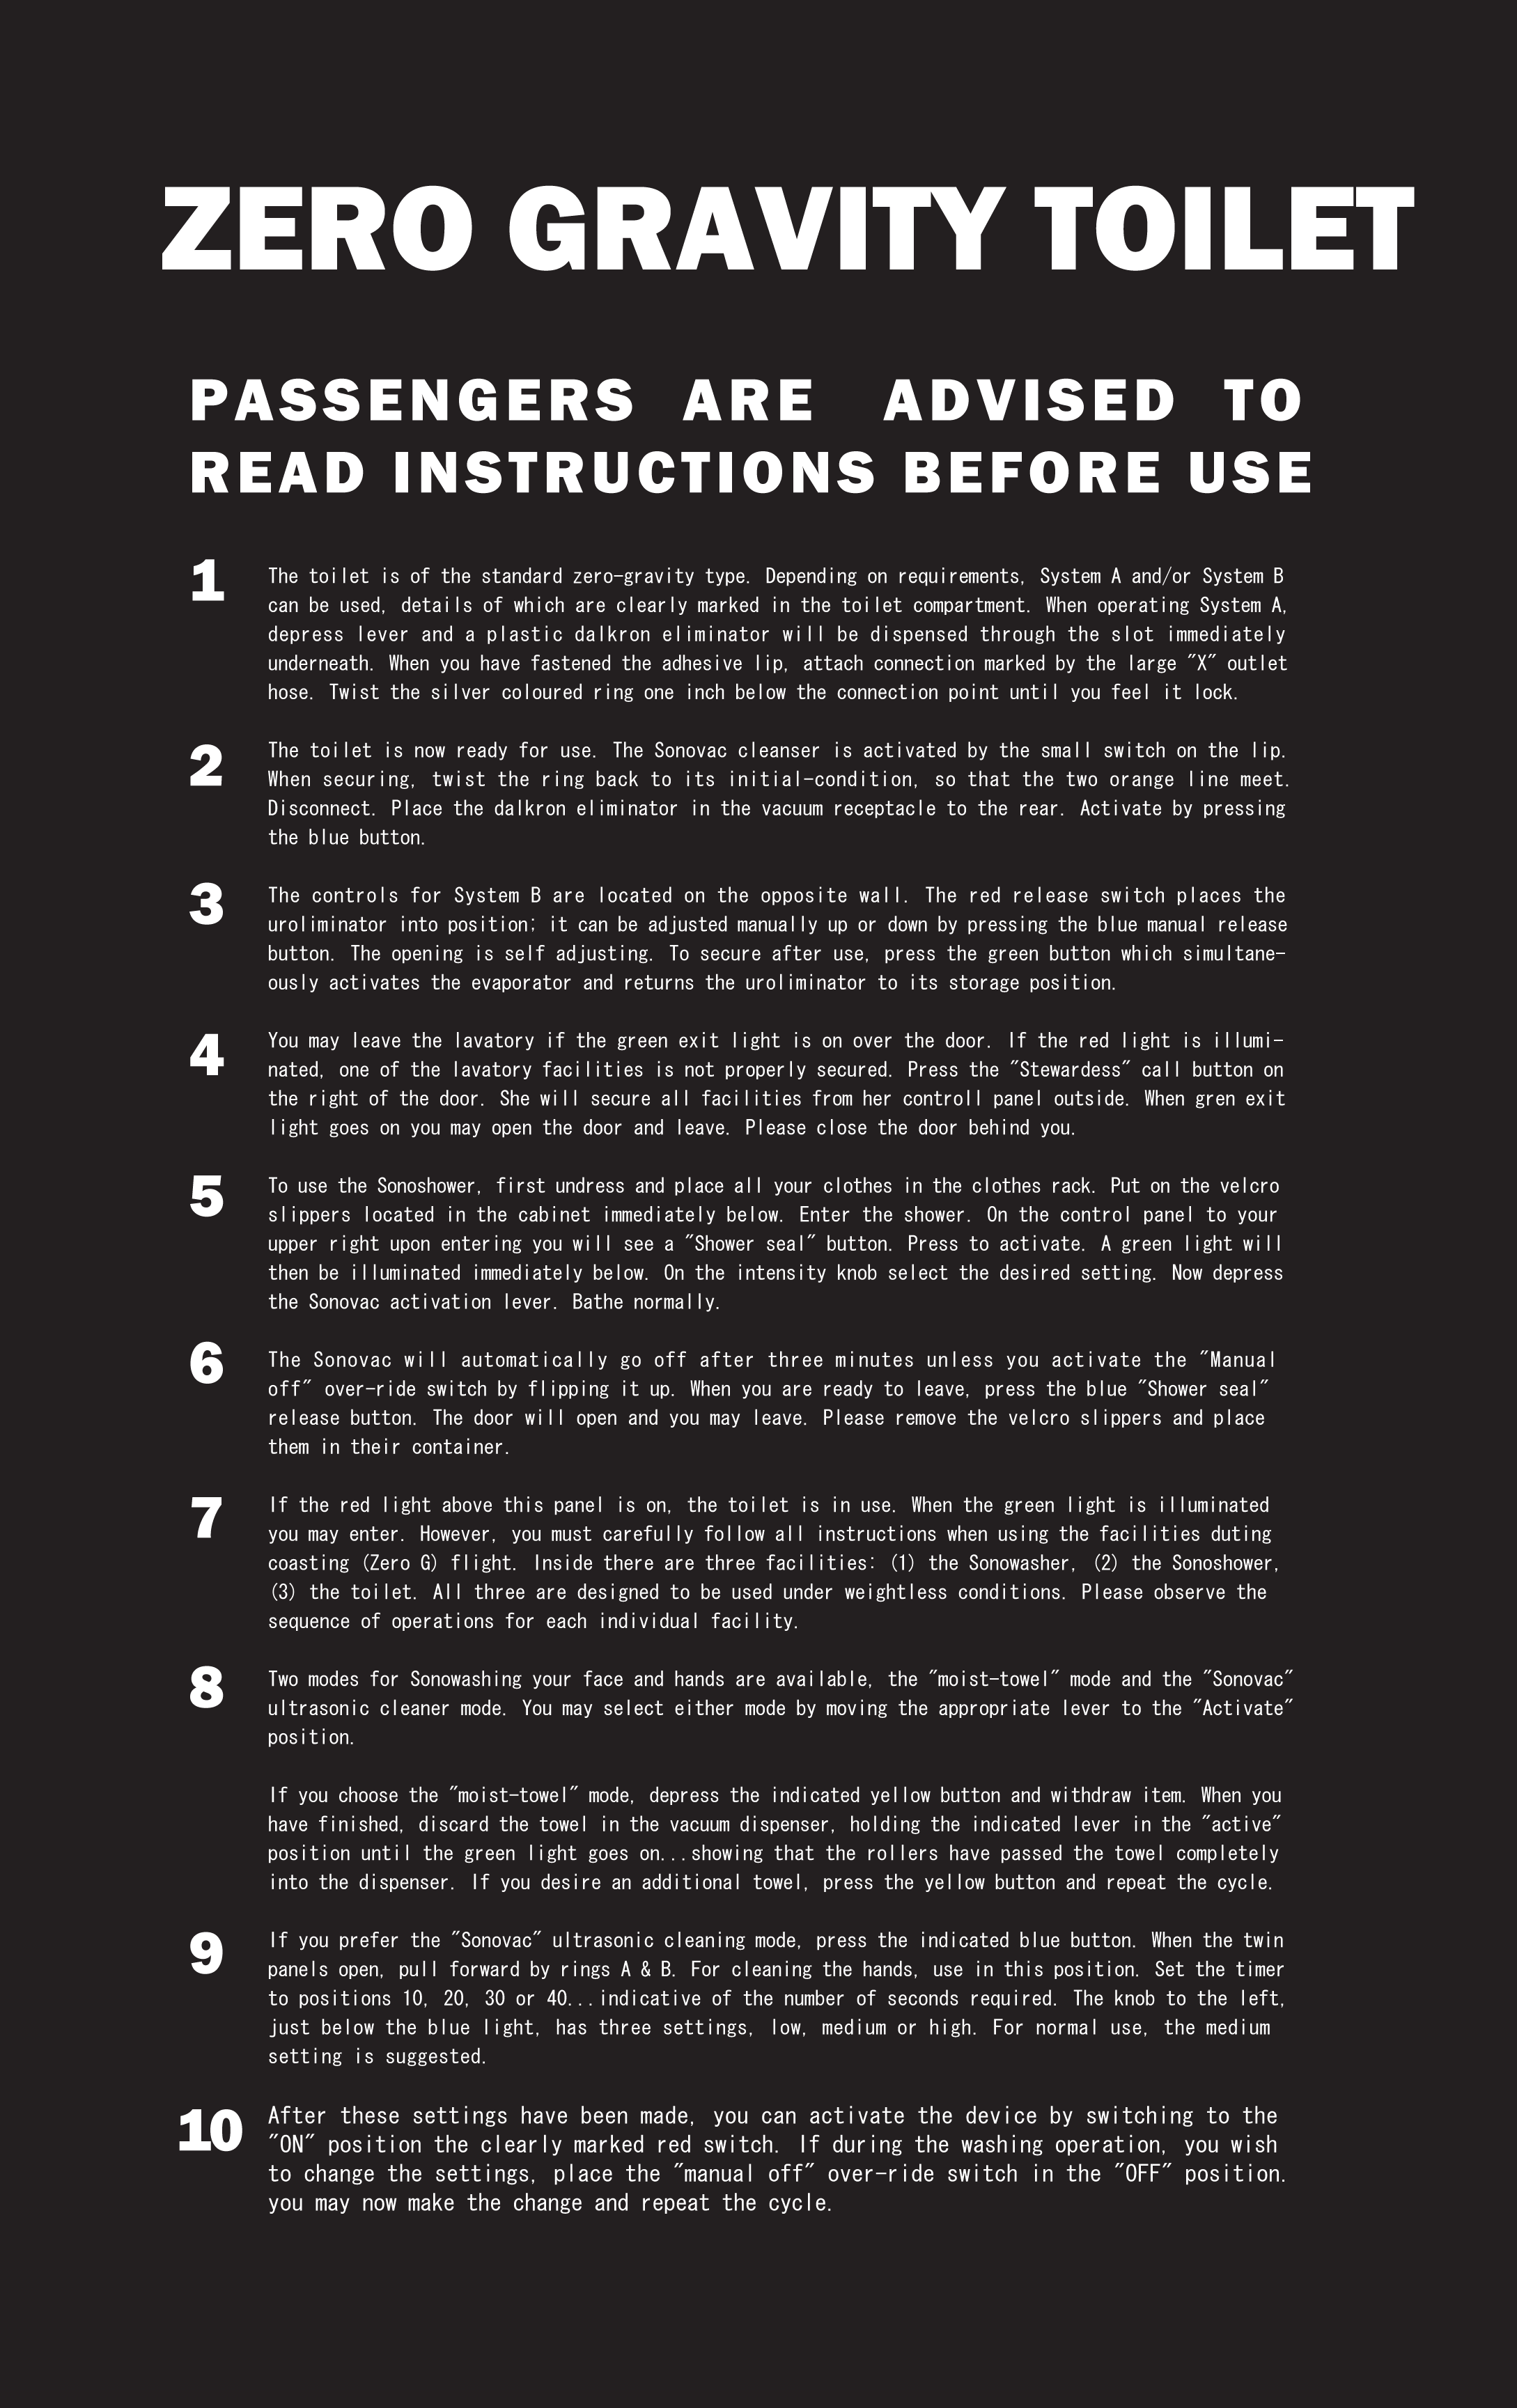
\includegraphics[scale=0.08]{img/002.png}
		\caption{Lista di istruzioni della toilette}
		\label{fig: 002}
	\end{center}
\end{figure}

\noindent\rule{\textwidth}{1pt}
\begin{center}
	\textbf{Toilette di Floyd}
\end{center}

Tendenza del progettista a complicare affari semplici e a pretendere che basti descrivere una procedura per renderla ovvia a qualsiasi utente.

\noindent\rule{\textwidth}{1pt}

\section{Sei concetti centrali}
\paragraph{Definizione classica di interazione (ISO 9241)} \label{par: ISO 9241}
\textbf{Un sistema interattivo} è una combinazione di componenti hardware e software che ricevono input da un utente umano e gli forniscono un output allo scopo di supportare l'effettuazione di un compito.

\begin{figure}[h!]
	\begin{center}
		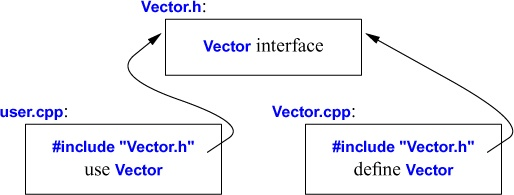
\includegraphics[scale=0.5]{img/003.jpg}
		\caption{Mappa sullo scopo e sul metodo di completamento di un'azione}
		\label{fig: 003}
	\end{center}
\end{figure}

\textbf{Un'interfaccia} è l'insieme dei componenti di un sistema interattivo (software o hardware) che forniscono all'utente informazioni e comandi per permettergli di effettuare specifici compiti attraverso il sistema. \label{par: sistema interattivo}

In comune hanno il concetto di "effettuazione di un compito", da ciò si capisce che il sistema interattivo permette all'utente di conseguire un'obiettivo (compito).

\subsection{Visibilità}
Permette all’utente di individuare facilmente qual è la funzione dell’oggetto, e quindi riconoscere se è adatto allo scopo prefissato. È il risultato dell’applicazione di tutti gli altri principi elencati.

\subsection{Modello concettuale}
É il modello che l’utente ha dell’oggetto in questione; il modello può essere superficiale e riferirsi alla sola conoscenza di relazione tra input e output, ma può anche essere più approfondito, arrivando a conoscere anche tutti i passaggi intermedi a livello macchina. Più il modello concettuale è fedele al funzionamento reale, maggiore è la probabilità di successo nell’interazione tra utente e macchina.

\subsection{Affordance (invito all’uso)} 
Vedere pagina \pageref{par: affordance}.

Gibson: è la risorsa o supporto che l'ambiente offre all'utente

Norman: è una qualsiasi proprietà o qualità di un oggetto che definisce i suoi possibili utilizzi o rende chiaro come possa o debba essere usato.

Una affordance è qualsiasi proprietà di un oggetto che invita una persona competente all'azione mediata da tale oggetto.

\subsection{Significanti}
Tutto ciò che aggiunge ulteriori indicazioni sull’esecuzione dell’azione, come direzione di movimento, senso di rotazione, ecc.

\subsection{Feedback (reazione)}
É l’insieme di risposte che il sistema comunica all’utente, in base alle azioni effettuate fino a quel momento.

\subsection{Mapping} 
Vedere pagina \pageref{par: mapping}.
	
É il rapporto fra i comandi, il loro azionamento ed i risultati che ne derivano nel mondo esterno; permette all’utente di creare un collegamento diretto fra i comandi di controllo e le parti dell’oggetto di cui modificano rispettivamente lo stato.



\section{Affordance} \label{par: affordance}
\noindent\rule{\textwidth}{1pt}
\begin{center}
	\textbf{Affordance (invito all’uso)}
\end{center}
Gibson: è la risorsa o supporto che l'ambiente offre all'utente

Norman: è una qualsiasi proprietà o qualità di un oggetto che definisce i suoi possibili utilizzi o rende chiaro come possa o debba essere usato.

Una affordance è qualsiasi proprietà di un oggetto che invita una persona competente all'azione mediata da tale oggetto.

\noindent\rule{\textwidth}{1pt}

Ci sono vari tipi di affordance:
\begin{itemize}
	\item \textbf{Cognitive}: aiuta gli utenti attraverso le loro capacità cognitive (pensare, decidere, imparare, ricordare e conoscere)
	\item \textbf{Fisiche}: aiuta l'utente attraverso le sue azioni fisiche (cliccare, toccare, puntabile, gesticolare, muovere)
	\item \textbf{Sensoriali}: aiuta l'utente attraverso le sue azioni sensoriali (vedere, sentire e percepire
	\item \textbf{Funzionali}: aiuta l'utente a realizzare il suo compito e a comprendere come usare lo strumento
	\item \textbf{Emotiva}: aiuta l'utente ad esperire certe emozioni (il caso più intuitivo è quello delle emoticon e delle sue evoluzioni) 
	\item \textbf{Sociale}: aiuta l'utente ad esperire certe funzioni sociali
\end{itemize}

Le affordance non sono esclusive, posso copartecipare all'intuizione, il problema è quando sono in contraddizione. Nel caso la progettazione non sia intuitiva gli utenti possono aggiungerle (ad esempio inserendo un cartello).

\section{Mapping} \label{par: mapping}
\noindent\rule{\textwidth}{1pt}
\begin{center}
	\textbf{Mapping}
\end{center}	
É il rapporto fra i comandi, il loro azionamento ed i risultati che ne derivano nel mondo esterno; permette all’utente di creare un collegamento diretto fra i comandi di controllo e le parti dell’oggetto di cui modificano rispettivamente lo stato.

\noindent\rule{\textwidth}{1pt}
\begin{figure}[h!]
	\begin{center}
		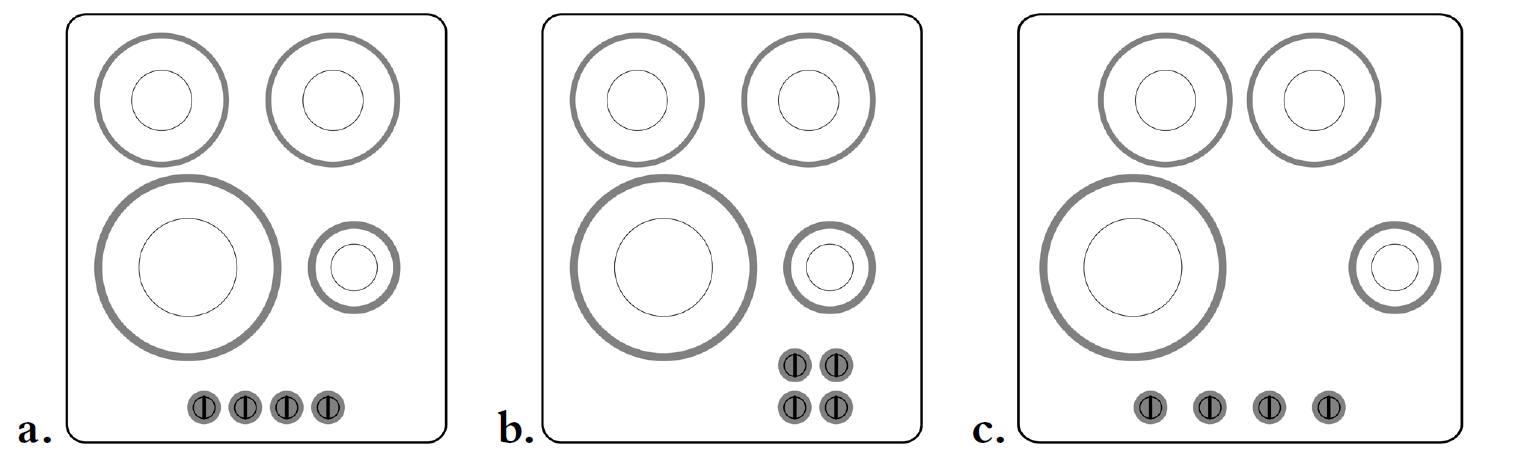
\includegraphics[scale=0.2]{img/006.png}
		\caption{Esempi di mapping topologici mancati e riusciti}
		\label{fig: 006}
	\end{center}
\end{figure}
Come possiamo vedere nell'immagine \ref{fig: 006} il mapping topologico è buono ma quello funzionale, in certi casi, può essere migliorato: cosa ha a che fare la rotazione con l'intensità della fiamma e quindi il calore?

\begin{figure}[h!]
	\begin{center}
		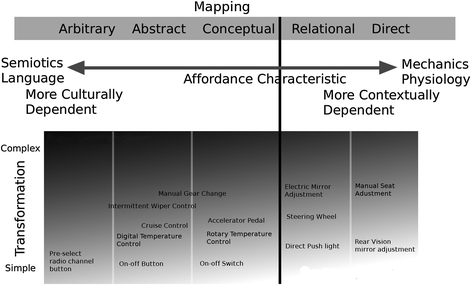
\includegraphics[scale=0.6]{img/007.png}
		\caption{Grafico mapping-affordance}
		\label{fig: 007}
	\end{center}
\end{figure}
Anche per il mapping possiamo averne di semplici e complessi. Dall'immagine \ref{fig: 007} possiamo vedere i tipi di mapping individuati da McLuhan:
\begin{itemize}
	\item \textbf{Arbitrario}: una relazione del tutto immaginata dal progettista e che l'utente adotta solo per prove ed errori e poi impara a memoria, senza riferimenti culturali o indicazioni fisiche
	\item \textbf{Convenzionale}: la relazione tra controllo ed effetto è stabile, quasi ovvia, ma legata a delle convenzioni. Ad esempio solo una convenzione ci permette di capire che la seconda marcia, che in molte automobili si trova nella fila inferiore e comunque sotto la prima marcia, in altre invece sopra, è quella che riduce la coppia alla ruota a parità di coppia del motore
	\item \textbf{Naturale}: la relazione è meno immediata che nel caso diretto (ma i concetti sono molto simili)
	\item \textbf{Diretto}: c'è una relazione fisica, visibile, spesso legata alla posizione, tra controllo (che afforda una azione) e l'effettore controllato che produce un effetto nel mondo
\end{itemize}

Ricordiamo che non si può avere mapping senza affordance ma si può avere affordance senza mapping.

Un'affordance non è solo qualcosa che suggerisce una azione su di essa ma anche qualcosa che suggerisce un possibile effetto sul mondo. è proprio il mappinga, che è una caratteristica dell'affordance, che si occupa di rendere questo collegamento o relazione più o meno semplice da capire.

\subsection{La legge di Fitt}
\noindent\rule{\textwidth}{1pt}
\begin{center}
	\textbf{Legge di Fitts}
	
	$MT = a + b\log_{2}(\dfrac{D}{W} + 1)$ \\dove MT è il tempo di movimento, D è la distanza dall'obiettivo e W è la grandezza dell'obiettivo
\end{center}
\begin{figure}[h!]
	\begin{center}
		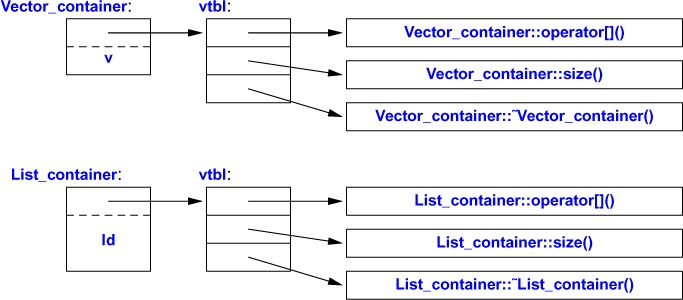
\includegraphics[scale=0.6]{img/004.jpg}
		\caption{Legge di Fitt}
		\label{fig: 004}
	\end{center}
\end{figure}
\noindent\rule{\textwidth}{1pt}

Nella progettazione si può pensare di rendere più efficienti per la legge di Fitt le funzioni più frequenti e rendere meno efficienti quelli per i quali serve una forma di sicurezza.

\section{Scheumorfismo}
Uno scheumorfismo è un ornamento fisico o grafico apposto su un oggetto allo scopo di richiamare le caratteristiche estetiche di un altro. Un esempio è la calcolatrice digitale che cerca di replicare gli schemi che ritroviamo su quelle fisiche, oppure all'applicazione di un e-reader che simula il girare fisicamente la pagina.

\begin{figure}[h!]
	\begin{center}
		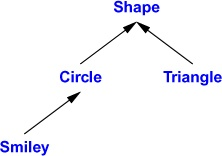
\includegraphics[scale=0.6]{img/005.jpg}
		\caption{Esempio di scheumorfismo}
		\label{fig: 005}
	\end{center}	
\end{figure}

Perchè oggi non viene più usato così pervasivamente? Perchè spesos questo approccio può essere estremamente utile per permettere all'utente un'interazione veloce ma porta con sè eventuali costi di performance. Oggi è stato sostituito da un approccio più flat. 

Lo scheumorfismo può anche portare il problema di essere vincolati troppo dall'oggetto fisico.

\section{Vincoli e workaround}\label{par: workaround}
Un vincolo può essere:
\begin{itemize}
	\item \textbf{passivo/concettuale}: ad esempio concepisco un form con tre campi e non quattro, per vincolare l'inserimento di soli tre tipi di dato; non prevedo un campo "note", non prevedo un canale di ritorno (feedback) tra consumatore e azienda
	\item \textbf{attivo/funzionale}: ad esempio concepisco dei controlli per cui l'utente non può proseguire se non compila tutti i campi, o non li compila "correttamente" sulla base di regex come ad esempio per l'indirizzo mail o il codice fiscale)
\end{itemize}

I vincoli vanno sempre bene? No, se l'utente si sentisse troppo vincolato potrebbe iniziare a creare dei workaround. Questi vengono chiamati "desire path".

\noindent\rule{\textwidth}{1pt}
\begin{center}
	\textbf{Desire Path}
\end{center}

Qualsiasi azione relativa all'esecuzione di un processo o di un compito (supportati dal sistema informatico) che non è prevista o descritta nei manuali di uso del sistema informatico e/o nei manuali che descrivono tale processo o procedura e che può bypassare l'uso del sistema o piegarlo ai propri fini.

"Percorso del desiderio", sono quei percorsi di interazione che descrivono il percorso ideale da parte dell'utente.

\noindent\rule{\textwidth}{1pt}

\section{Progettare per affordance} \label{par: complessità}
\begin{itemize}
	\item Seguire le maggiori convenzioni già stabilite per immagini e azioni ed adottare un mapping naturale il più spesso possibile
	\item Se appropriato, usare parole in aggiunta alle icone e alle grafiche
	\item usare metafore riconoscibili (ad esempio il cestino dei rifiuti per indicare il cancellare un file)
	\item Essere consistenti e coerenti nell'uso dei modelli concettuali usati durante la fase di design (banalmente l'usare sempre la stessa dicitura per il tasto di conferma)
\end{itemize}

\begin{figure}[h!]
	\begin{center}
		
\includegraphics[scale=0.6]{img/008.jpg}
		\caption{Mappa complessità funzionale e strutturale}
		\label{fig: 008}
		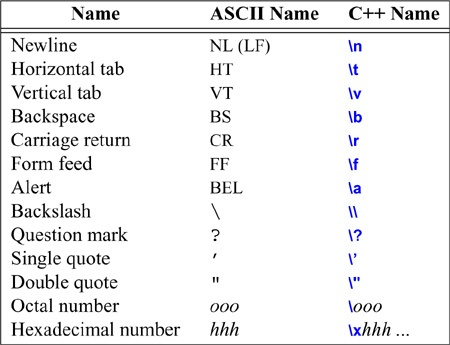
\includegraphics[scale=0.6]{img/009.jpg}
		\caption{Mappa complessità funzionale e d'uso}
		\label{fig: 009}
	\end{center}
\end{figure}
\begin{itemize}
	\item \textbf{Complessità funzionale}: indica quante funzioni possono essere svolte tramite l'interfaccia in analisi (un cacciavite a punta singola ha una bassa complessità funzionale, un coltellino svizzero ha un'alta complessità funzionale in quanto in base a come viene usato può svolgere numerose funzioni in virtù delle sue componenti)
	\item \textbf{Complessità strutturale}: indica, genericamente, quanto sia complessa la struttura di uno strumento (un cucchiaio ha una complessità strutturale bassa, uno smartphone una complessità strutturale alta)
	\item \textbf{Complessità d'uso}: indica quando sia semplice utilizzare l'interfaccia, ha un forte elemento basato anche sulle capacità personali (una maniglia ha complessità d'uso bassa, una macchina con cambio manuale ha complessità d'uso alta)
\end{itemize}

Il nostro obiettivo è raggiungere alta complessità funzionale con bassa complessità d'uso. Ci sono degli accorgimenti che ci permettono di diminuire la complessità d'uso, ad esempio una progettazione oculata.

\subsection{Perchè è necessario semplificare l'uso?}
Prima di tutto la pervasività della tecnologia al giorno d'oggi ci richiede ciò, se fosse complicata da usare ci sarebbero più difficoltà nella sua implementazione nella vita di tutti i giorni.

L'accessibilità è un altro capo saldo, renderla usabile e accessibile a tutti, non solo in termine di rimozione di barriere architettoniche ma in generale come possibilità d'accesso, non bloccata da limiti fisici o di disponibilità.

C'è anche la necessità di comprendere ruoli e possibilità della tecnologia per migliorare la qualità della vita.

Le interfacce non sono solo il mezzo interattivo con i sistemi ma sono anche un filtro della complessità d'uso, una buona interfaccia semplifica l'utilizzo e da qua l'integrazione. La capacità di creare un sistema con una minore complessità d'uso ci permette di essere competitivi.

\chapter{Valutazione di usabilità}
\section{In cosa consiste il progetto?}
\textbf{Chi è coinvolto}? Noi e utenti reali

\textbf{Che tipi di analisi ci sono?}
\begin{itemize}
	\item Confronto longitudinale: nel tempo
	\item Confronto trasversale: tra due opzioni
\end{itemize}
\textbf{Quali sono gli step?}
\begin{figure}[h!]
	\begin{center}
		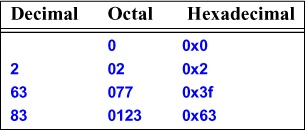
\includegraphics[scale=0.55]{img/010.jpg}
		\caption{Gli step per i due confronti}
		\label{fig: 010}
	\end{center}
\end{figure}
\textbf{Valutazione euristica}: 3 utenti esperti di dominio + 3 utenti esperti di usabilità (cioè noi). Per utenti esperti di dominio si intendono utenti che usano abitualmente il tipo di interfaccia in analisi.

\textbf{User test}: i 12 utenti tra i 24 che saranno coinvolti negli user test devono essere più rappresentativi possibili della popolazione utilizzatrice.

Durante lo user test bisogna registrare l'interazione (c'è un modulo apposito per la privacy).

\section{Valutazione euristica (qualitativa)} \label{par: euristica}
Si coinvolgono utenti (esperti del task) e/o esperti di usabilità (inclusi noi stessi).

Per valutare sistemi interattivi, a qualsiasi livello di prototipazione e maturità alla luce dei principi di buona progettazione.

Qualitativa non si intende in modo vago ma dove non viene prodotto un numero come output ma invece farsi un'idea sufficientemente completa dei possibili problemi di usabilità.

\begin{figure}[h!]
	\begin{center}
		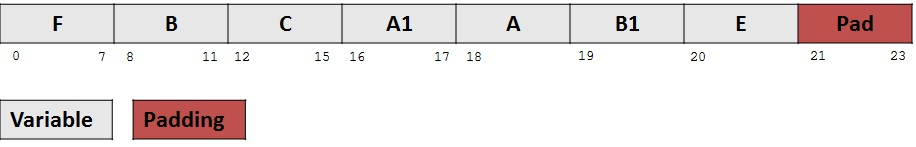
\includegraphics[scale=0.6]{img/012.jpg}
		\caption{Mappa expertise}
		\label{fig: 012}
	\end{center}
\end{figure}
Per tutti gli utenti bisogna includere all'interno della relazione una mappa che interpoli expertise di dominio e sulla usabilità e posizioni gli utenti coinvolti su di questa (una mappa come nella figura \ref{fig: 012}.

L'expertise sull'usabilità è quella riguardante cosa si conosce dei buoni principi di progettazione, quella sul dominio è l'expertise nell'applicazione specifica.

La valutazione euristica è la valutazione (di usabilità) svolta alla luce di un determinato insieme di euristiche (ben definite, possibilmente ben note, prese a riferimento) per identificare soluzioni di design che o si conformano o violano una o più euristiche di tale insieme.

\subsection{Quali indicazioni per il design dell'interfaccia utente?}
\begin{figure}[h!]
	\begin{center}
		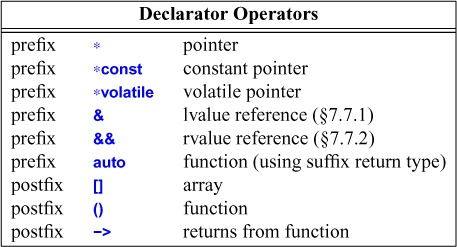
\includegraphics[scale=0.6]{img/013.jpg}
		\caption{Tipi di principi e linee guida}
		\label{fig: 013}
	\end{center}
\end{figure}

Si chiamano anche principi euristici o semplicemente "euristiche". Una euristica è quindi un insieme di concetti, riferimenti e, soprattutto, strategie che si sono rilevate particolarmente adatte a risolvere un determinato problema, nel nostro caso la progettazione di sistemi interattivi usabili.
\subsubsection{Principi}
Indicazioni generali per la progettazione di interfacce utente usabili, basate su evidenza scientifica o sul generale consenso. Derivano dalla conoscenza degli aspetti psicologici, computazionali e sociali e sono indipendenti dalla tecnologia. Sono espressi spesso in forma molto generale.

\subsubsection{Standard}
Insieme di regole da applicare nel progetto di una classe di sistemi. possono essere vincolanti. Sono di norma emesse da un Ente di standardizzazione (e.g. ISO). La conformità allo standard deve essere valutabile in modo preciso. (Vedere \pageref{par: ISO 9241}

\subsubsection{Linee guida e design patterns}
Insieme di raccomandazioni per il progetto dell'interfaccia utente per una particolare classe di sistemi, espresse in modo generale ma meno astratte dei principi, con esempi e motivazioni. Non sono mai vincolanti, sta al progettista decidere sulla opportunità per applicarle caso per caso.

Il concetto di "design pattern" nasce in architettura. Si tratta di riutilizzare buone pratiche (appunto raccomandazioni) per non dovere reinventare tutto da capo. Per i programmatori i più famosi sono \href{https://refactoring.guru/design-patterns}{i design pattern pensati dalla GoF}. Diffondono standard testati e facilitano la formazione di un linguaggio comune.

\subsubsection{Regole di progetto}
Insieme di regole o specifiche da applicare nel progetto di un particolare sistema. Sono vincolanti all'interno del progetto, ad esempio perchè dettate da precisi requisiti del cliente/committente o per motivi di budget e vincoli progettuali.


Si usano i principi e non le linee guida perchè non vogliamo essere vincoli eccessivi. 
\subsection{Livelli di autorevolezza dei principi}
Ci sono diversi livelli di autorevolezza dei principi (o forza dell'evidenza):
\begin{enumerate}
	\item Completamente supportati da risultati di ricerca e dati empirici
	\item Basati su pratica generalmente accettata (in modo documentato)
	\item Non ben documentate, ma supportate dall'opinione di professionisti esperti
	\item Opinione individuale
\end{enumerate}

Solo i primi due gradi sono recepiti. I principi di Nielsen sono tra B e C, alcune soluzioni specifiche (ispirate a quei principi) anche di livello A.

\subsection{Le euristiche usate più frequentemente}
La prima checklist è la \href{https://ixdchecklist.com/}{IXD checklist}, utile per la valutazione di siti web che vogliono essere anche gradevoli visivamente. Viene creata una lista di ambiti e in ognuno di questo ci sono vari domini ai quali si applicano:
\begin{itemize}
	\item Euristiche
	\begin{itemize}
		\item Affordance
		\item Feedback
		\item Simplicity
		\item Structure
		\item Consistency
		\item Tolerance
		\item Accessibility 
	\end{itemize}
	\item Domini
	\begin{itemize}
		\item Interface
		\item Iconography
		\item Typography
		\item Interaction
		\item Navigation
	\end{itemize}
\end{itemize}

Questa checklist è altamente generica ma permette di raggruppare le idee e scovare problemi di usabilità da migliorare.

Un altro standard è l'ISO 9241-110 che prescrive 7 principi del dialogo uomo macchina:
\begin{itemize}
	\item Adeguatezza del compito
	\item Autodescrizione (capacità del sistema di dire in che stato sia)
	\item Conformità alle aspettative dell'utente
	\item Adeguatezza all'apprendimento (facilitare l'adozione facilitando il processo di apprendimento)
	\item Controllabilità
	\item Tolleranza verso gli errori
	\item Adeguatezza alla personalizzazione (inteso come fine tuning)
\end{itemize}

\subsubsection{Euristiche di Nielsen}
L'insieme più importante e a cui viene attribuita una buona autorevolezza sono le \href{https://www.neurowebdesign.it/it/alla-scoperta-delle-10-euristiche-di-nielsen/}{euristiche di Nielsen}. \\\underline{Possono essere tenute in sede d'esame}.
Basati su un'analisi fattoriale di 249 problemi di usabilità con cui si è derivato l'insieme minimo per massimizzare la potenza esplicativa.

In rete ci sono numerosi template per tenere traccia dei problemi.

Una rielaborazione del professor Mussio:
\begin{itemize}
	\item[] \textbf{Percezione}
	\begin{itemize}
		\item fare vedere lo stato del sistema (feedback)
		\item adeguare il sistema al mondo reale (parlare il linguaggio dell'utente)
		\item controllo dell'utente e libertà (uscite indicate chiaramente)
	\end{itemize}
	\item[] \textbf{Cognizione}
	\begin{itemize}
		\item assicurare consistenza (nell'applicazione, sistema, ambiente)
		\item riconoscimento piuttosto che uso della memoria dell'utente
		\item assicurare flessibilità ed efficienza d'uso (accelleratori)
		\item visualizzare tutte e sole le informazioni necessarie (estetica e design minimalista)
	\end{itemize}
	\item[] \textbf{Errori}
	\begin{itemize}
		\item prevenire gli errori
		\item permettere all'utente di correggere gli errori e non solo di rilevarli
		\item help contestuale e documentazione
	\end{itemize}
\end{itemize}

\subsection{Spiegazione euristiche}
\subsubsection{Fare vedere lo stato del sistema (feedback)}
\begin{itemize}
	\item Il sistema deve informare continuamente l'utente di ciò che sta facendo e come sta interpretando gli input dell'utente.
	\item L'utente deve poter capire l'effetto dell'azione passata sullo stato presente e individuare le possibili nuove azioni.
	\item Fornire indicazioni sui malfunzionamenti e le ipotesi plausibili delle cause. Non bisogna segnalare solo per errori ma anche se l'applicazione è in uno stato di transizione, ad esempio cambiare il cursore durante un'elaborazione
	\item Espresso in maniera concreta, non astratta o in termini generali (ad esempio copia file ma quale file da dove a dove)
	\item Il feedback può avere differenti gradi di persistenza. Esempi:
	\begin{itemize}
		\item \textbf{Persistenza breve}: un messaggio che la stampante ha finito la carta
		\item \textbf{Persistenza media}: sta sullo schermo finchè l'utente esplicitamente non lo riconosce, ad esempio l'avviso di reindirizzamento su di un'altra stampante
		\item \textbf{Persistenza alta}: rimane una parte permanente dello schermo, ad esempio la batteria
	\end{itemize}
	\item è importante nel caso di operazioni che richiedono una lunga elaborazione
\end{itemize}

\subsubsection{Adeguare il sistema al mondo reale (parlare il linguaggio dell'utente)}
\begin{itemize}
	\item Permettere all'utente di sfruttare la sua esperienza nell'interagire con il sistema
	\item Familiarità: adotta le notazioni di utente, convenzioni sui nomi
	\item Proiezione mondo reale: metafore familiari
	\item I dialoghi, se possibile, devono essere nella lingua nativa dell'utente così come le icone devono rispettare la cultura (affordance percepita)
\end{itemize} 

\subsubsection{Controllo dell'utente e libertà (uscite indicate chiaramente)}
\begin{itemize}
	\item Gli utenti non si devono sentire "intrappolati" dai computer, deovno sentire che sono loro che controllano il dialogo: ad esempio usare le finestre modali solo quando servono
	\item Offrire sempre all'utente un modo semplice per uscire dalla situazione corrente, dare delle chiare vie d'uscita
	\item Offrire sempre delle possibilità di "Undo", ovvero tornare indietro sui propri passi
	\item vie d'uscita e undo permettono all'utente di imparare esplorando il sistema (flip undo è il singolo step, multiple undo è quello che permette di navigare in vari step e solitamente è associato ad un redo)
	\item permettere di interrompere o cancellare operazioni che durano troppo
\end{itemize}

\subsubsection{Assicurare consistenza (nell'applicazione, sistema, ambiente)}
Avere la stessa interfaccia nei vari ambiti permette una veloce navigazione dell'applicazione. Avere i pulsanti ok, cancel, help messi sempre in posizione differente possono disorientare.

Nell'ambito del gruppo di sviluppo è importante adottare o definire convenzioni interne di rappresentazione e di interazione con rigore e farle rispettare in modo da avere una consistenza interna.

\subsubsection{Riconoscimento piuttosto che uso della memoria dell'utente}
Un comportamento corretto è quello di rimuovere la necessità per l'utente di ricordare le cose a memoria quando possono essere mostrate direttamente.

Se si richiede all'utente un formato specifico è meglio ricordarglielo e non lasciare che usi un sistema di try and error. Un modo è mostrare il pattern, un altro è riempire il campo con un placeholder. Nel caso ci sia un intervallo legale specificarlo.

\subsubsection{Assicurare flessibilità ed efficienza d'uso (accelleratori)}
L'utente esperto deve poter svolgere velocemente le operazioni più frequenti, ad esempio l'uso di shortcuts (accelleratori).

Flessibilità nel senso che il sistema deve permettere di fare le stesse cose in maniere diverse (ad esempio per un utente novizio o esperto)

Altri esempi:
\begin{itemize}
	\item Segnalibri
	\item Breadcrumb trail
	\item Uso della storia dell'interazione (e.g. file aperti di recente)
	\item Definizione di templates e macro
	\item Type-ahead (poter inserire il prossimo input prima che il computer sia pronto ad accettarlo)
	\item Fornire valori di default
\end{itemize}

\subsubsection{Visualizzare tutte e sole le informazioni necessarie (estetica e design minimalista)}
L'interfaccia deve essere semplice e gradevole e rispecchiare nella maniera più naturale possibile i compiti dell'utente. Presentare solo l'informazione:
\begin{itemize}
	\item che l'utente vuole
	\item quando l'utente la vuole
	\item come l'utente la vuole
	\item dove l'utente la vuole
\end{itemize}
e non accompagnata da informazioni non rilevanti o fuorvianti.

Raggruppare poi le informazioni che vengono usate insieme e presentarle in modo da suggerire la sequenza di azioni.

\paragraph{Una credenza errata}
"Più opzioni offro e più modi di fare le cose metto a disposizione, più utenti soddisfo" (noto come Bells and whistles bias). Ogni volta che si aggiunge un'opzione l'utente ha una cosa in più da ricordare e da usare in maniera scorretta.

Un'alternativa: offrire diversi "modi utente", ad esempio per novizio, esperto, operatore di linea e manutentore...

Il fenomeno del low use riguarda il rapporto tra funzioni usate spesso o a volte e quelle che non sono note o sono note ma inutilizzate. Si può calcolare un "use index" così:
$$UI=\dfrac{(N_{S}*1) + (N_{A}*0,5) + (N_{M}*0)}{N_{S}+N_{A}+N_{M}}$$

Dove:
\begin{itemize}
	\item[] $N_{S}$ sono le funzioni usate spesso
	\item[] $N_{A}$ sono le funzioni usate a volte
	\item[] $N_{M}$ sono le funzioni mai usate
\end{itemize}

\begin{center}
I low users sono quelli con $$UI \leq 0,5$$
\end{center}

Può essere usato per capire quali funzioni promuovere e, nel caso, potenziare.

\paragraph{Importanza della grafica, del layout e del colore (estetica)}
Mettere "prima" le informazioni che devono essere lette prima.

Oggetti lampeggianti o CARATTERI MAIUSCOLI, solo se necessario, anche perchè rallentano del 10\% la velocità di lettura.

In generale si considera una lettura media di 200-300 pam (parole al minuto) per la lettura generica (rounding) ma la velocità dipende dal task (memorizzazione 100, skimming 700), dall'illuminazione, dai font, dal livello di scolarità.

Considerare alcuni problemi aiuta, ad esempio per il daltonismo:
\begin{itemize}
	\item Non usare più di 5-7 colori
	\item Rendere l'interfaccia distinguibile anche senza colori
	\item Non dedicare troppo spazio al titolo, nome del venditore, numero di versione e informazioni simili.
\end{itemize}

\subsubsection{Prevenire gli errori}
\begin{itemize}
	\item Individuare le situazioni di possibile errore e cercare di aiutare l'utente. Cerare meccanismi di prevenzione, ad esempio selezionare i valori da un menù e non tramite digitazione libera.
	\item Usare le richieste di conferma.
	\item Evitare comandi troppo simili con significati diversi.
	\item Creare meccanismi di comunicazione utente - progettista: errori rilevati dall'utente e inviabili tramite log al progettista.
\end{itemize}

\paragraph{Tecniche di prevenzione}
\begin{itemize}
	\item Diversificare le azioni dell'utente
	\item Amodalità: si intende fare sì che i comandi non abbiano significato differente in base alla modalità utente
	\item Funzioni vincolate
	\item Avvertimenti e richieste di conferma
	\item Default inoffensivi
	\item Bypass sicuri (e.g. password dimenticata)
\end{itemize}

\subsubsection{Permettere all'utente di correggere gli errori e non solo di rilevarli}
Dare buoni messaggi di errore è essenziale, devono essere chiari, senza codici, dare indicazioni precise, proporre una soluzione e, soprattutto, essere gentili.

La recoverability è la capacità di raggiungere il risultato voluto dopo avere commesso l'errore. Se un'azione non è reversibile sarebbe meglio renderla difficilmente conseguibile (inefficienza programmata).

\paragraph{Granularità dei messaggi d'errore}
Meglio un messaggio d'errore alla volta quando viene commesso l'errore o tutti insieme alla fine?

\subsubsection{Help contestuale e documentazione}
Il sistema perfetto è così facile da usare che non ha bisogno di help e manuali ma poichè non esiste è sempre bene prevederli.

Bisogna anche tenere a mente che spesso gli utenti non leggono i manuali, preferiscono usare il sistema senza avere letto alcuna spiegazione, quindi mai dare per presupposto che l'utente abbia letto il manuale e fornire aiuti in linea con documentazione raggiungibile in modo preciso.

L'help deve essere minimale e contestuale (Clippy non era male).


\subsection{AB testing}
\begin{figure}[h!]
	\begin{center}
		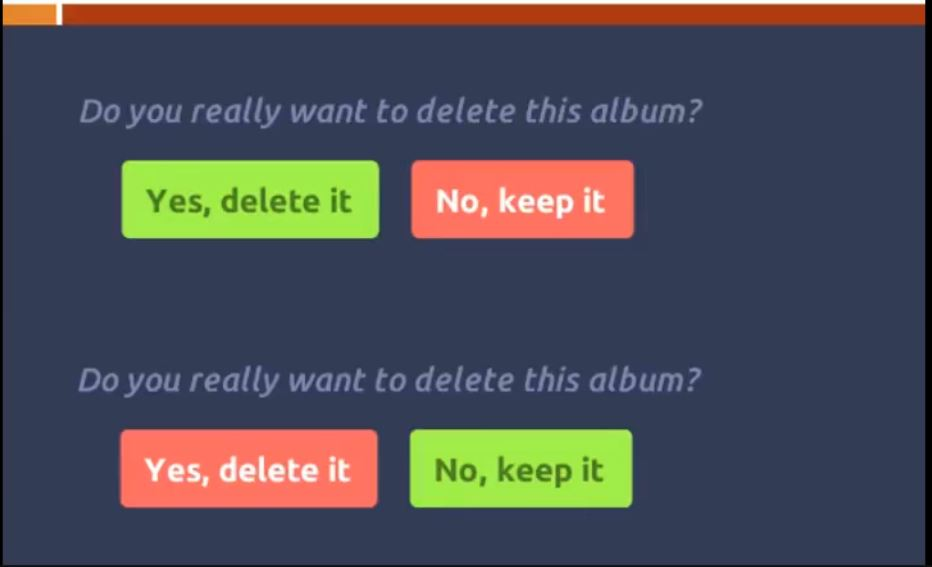
\includegraphics[scale=0.6]{img/019.jpg}
		\caption{Esempio di AB testing}
		\label{fig: 019}
	\end{center}
\end{figure}
Presentare due alternative di design e fare scegliere agli utenti quale preferiscano permette di capire quale sia l'interazione statisticamente preferita.

AB suggerisce due possibilità ma in realtà possono esserci N combinazioni di elementi sotto esame, ad esempio combinazioni di media, label dei pulsanti, colori ecc. che vengono proposti agli utenti e poi valutati in base ad un feedback misurabile.

\subsection{Manuali d'uso}
I manuali non vengono mai letti prima ma solo quando si conosce già il sistema e si devono risolvere problemi specifici. Quindi, progettiamo le cose in modo da poterne fare a meno nelle fasi iniziali.

\section{Valutazione euristica di usabilità}
è una tecnica sistematica di ispezione predittiva (non misurazione).

Un gruppo di valutatori (e/o esperti) esamina il sistema e identifica eventuali problemi di usabilità rispetto ad un insieme prefissato di principi, le cosiddette euristiche. La valutazione può essere:
\begin{itemize}
	\item olistica (complessiva e non guidata) o task oriented\footnote{La differenza tra task e scenario è che un task è un compito da adempiere ma in maniera generale, scenario è invece un insieme prescrittivo di passi (nel Behavios-driven development è la sequenza \href{https://martinfowler.com/bliki/GivenWhenThen.html}{given when then})} (l'utente deve conseguire un obiettivo specifico)
	\item con o senza osservatori
\end{itemize}

Il risultato di una valutazione euristica è un elenco di problemi di usabilità, associati ad una o più euristiche, pesati per gravità.

\subsection{Sequenza di passi}
\begin{enumerate}
	\item scegliere un'applicazione
	\item concepire 2 o 3 task
	\item ogni persona nel gruppo base esplora l'applicazione (valutazione esperta olistica) con uno dei form a portata di mano
	\item ogni persona, indipendentemente dagli altri, scrive un elenco di problemi, riconducendoli alla violazione di una o più euristiche
	\item ora viene presentata l'applicazione a tre utenti esperti di domini. A loro viene dato un tempo di 3-4 minuti per esplorare l'applicazione (valutazione utente olistica). Deve essere comunicato che l'utente verrà registrato (con presentazione di modulo dedicato) e di pensare ad alta voce mentre usa l'applicazione (think aloud protocol analysis), esprimendo quello che gli piace e vuole fare e quello che non gli piace e non riesce a fare. Uno del gruppo base gli deve stare vicino, senza prendere appunti. Un altro prende appunti, segnandosi tempi ed espressioni verbali particolari (queste espressioni sono da inserire all'interno delle slide).
	\item presentare un task di quelli definiti al passo 2. Meglio farlo con una presentazione o filmaot che spieghi obiettivo e macropassi.
	\item fare eseguire all'utente il task (non più di 3-4 minuti, valutazione utente task based) e continuare con la protocol analysis. Se ha bisogno di aiuta la persona vicina gli dia suggerimenti
	\item dalla sessione di uso di ciascun utente estrarre collaborativamente un elenco di problemi di usabilità
	\item mettere insieme le liste individuali e quelle che sono state prodotte in sessione con gli utenti, decidendo cosa togliere e cosa lasciare
	\item predisporre un questionario con il quale prioritizzare noi e agli utenti i problemi trovati
	\item associare un problema ad una o più euristiche
\end{enumerate}

I task devono essere realistici, per fare alcuni esempi:
\begin{itemize}
	\item user goal: esplorare le offerte dei prodotti e acquistarne uno
	\item task concepito male: acquista un paio di scarpe da corsa della Nike arancioni
	\item task migliore: compra un paio di scarpe sotto i 40 euro
\end{itemize}

I task devono essere eseguibili:
\begin{itemize}
	\item user goal: cercare un film e i suoi orari
	\item task concepito male: vuoi vedere un film di domenica pomeriggio. Vai sul sito X e dimmi dove cliccheresti come prima cosa
	\item task migliore: usa il sito X per trovare un film che ti piacerebbe vedere di domenica pomeriggio
\end{itemize}

Evitare suggeritmenti e descrizioni dei singoli passi:
\begin{itemize}
	\item user goal: consultare i voti online
	\item task concepito male: vuoi vedere i voti del tuo esame IUM. Vai sul sito del corso, loggati e dimmi dove cliccheresti per vedere il tuo voto
	\item task migliore: cerca sul sito del corso il risultato dell'esame IUM
\end{itemize}

A fine progetto bisogna anche includere una matrice con una serie di dati che mettano assieme i problemi trovati e con che frequenza per poi identificare gli esaminatori migliori e i problemi più difficili:
\begin{figure}[h!]
	\begin{center}
		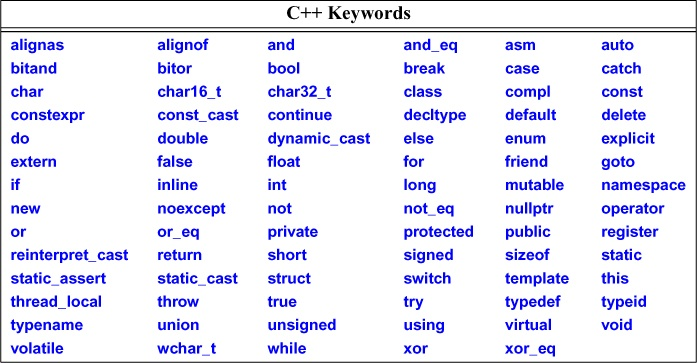
\includegraphics[scale=0.6]{img/014.jpg}
		\caption{Matrice problemi/utente}
		\label{fig: 014}
		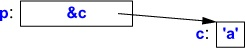
\includegraphics[scale=0.6]{img/015.jpg}
		\caption{Matrice problema/utente}
		\label{fig: 015}
	\end{center}
\end{figure}

\subsubsection{Scala di valutazione dei problemi}
\begin{itemize}
	\item[0] Non sono d'accordo che questo sia un problema di usabilità
	\item[1] \textbf{è solo un problema "cosmetico"}: non deve essere risolto a meno che nel progetto non sia disponibile del tempo extra 
	\item[2] \textbf{problema secondario}: alla sua risoluzione bisognerebbe dedicare bassa priorità
	\item[3] \textbf{problema rilevante}: è importante risolverlo, bisognerebbe dare alta priorità alla sua risoluzione
	\item[4] \textbf{catastrofe di usabilità}: è imperativo risolverlo prima che il prodotto possa essere rilasciato
\end{itemize}
Con questo specchietto si può prioritizzare la lista di problemi. Nel rapporto di severità bisogna riportare anche il numero di persone coinvolte in questa valutazione della severità.

Alcuni indicatori per la valutazione della gravità sono:
\begin{itemize}
	\item La frequenza o probabilità di occorrenza: è comune o raro?
	\item L'impatto del problema SE esso occorre: è facile o difficile da superare? Quali sono le conseguenze all'atto pratico?
	\item La persistenza: è un problema in cui lo stesso utente può incappare più volte anche essendone consapevole e a conoscenza o è di fatto una singola occorrenza?
\end{itemize}

\begin{figure}[h!]
	\begin{center}
		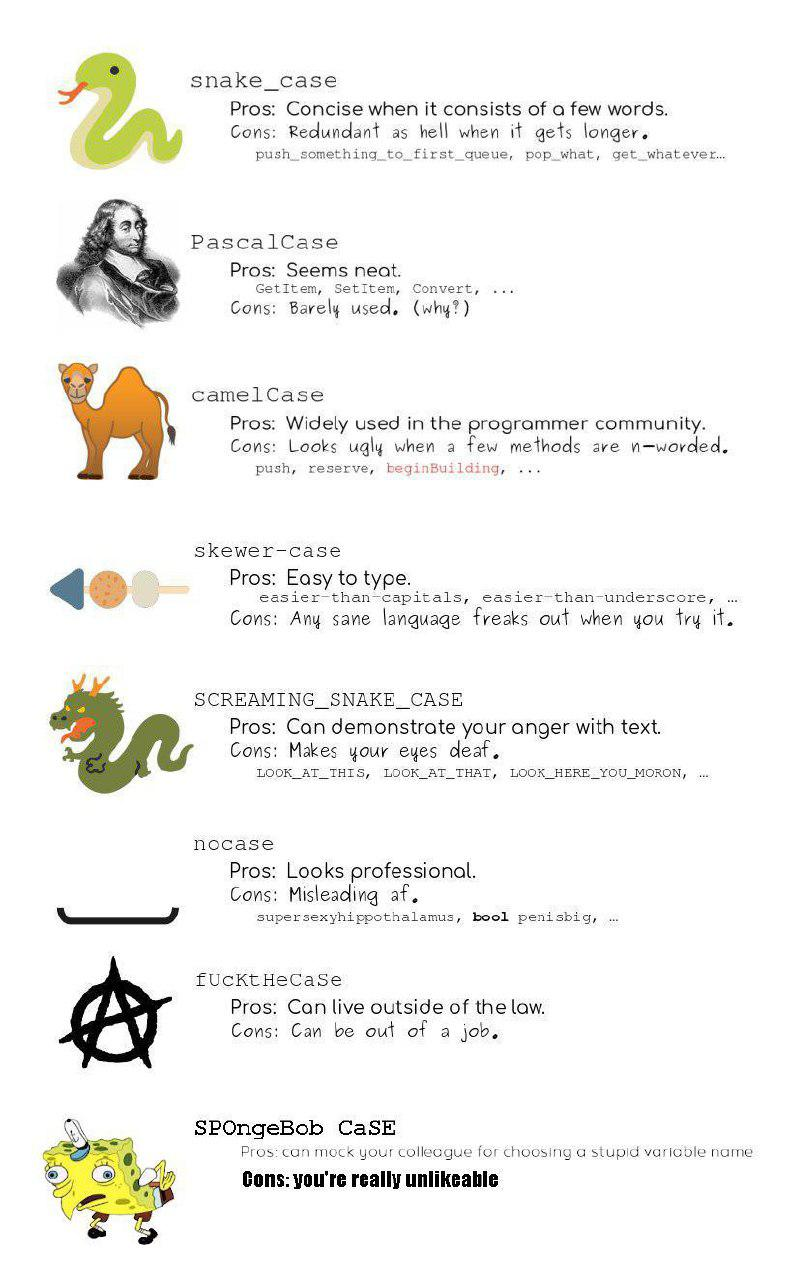
\includegraphics[scale=0.6]{img/016.jpg}
		\caption{Esempio di riassunto dei riscontri}
		\label{fig: 016}
	\end{center}
\end{figure}

\subsubsection{Perchè fare una valutazione euristica?}
è una tecnica dell'approccio più generale detto di "discount usability engineering" (veloce, efficiente, efficace). Nielsen ha riscontrato spesso rapporti benefit-cost > 1:50 (ovvero la valutazione costa 10k ma i benefici attesi sono stimati a 500k). Questi benefici derivano dalla non segnalazione di difetti, minore numero di rinunce da parte degli utenti.

\subsection{Valutazione euristica vs. test utente}
Pro della valutazione euristica: 
\begin{itemize}
	\item è più veloce (quindi meno costosa)
	\item i risultati sono già in forma interpretata
\end{itemize}

Contro:
\begin{itemize}
	\item meno accurata: può non individuare dei problemi o produrre falsi positivi
	\item non tiene conto degli utenti veri e dei loro compiti situati
\end{itemize}

\subsection{Valutazione euristica: risorse necessarie}
\begin{itemize}
	\item Un sistema funzionante oppure un prototipo o un mock-up.
	\item n valutatori
	\item un osservatore se vengono coinvolti utenti esperti
	\item tempo:
	\begin{itemize}
		\item In ambito professionale una sessione individuale di osservazione dura tra i 30 e i 90 minuti ma noi siamo autorizzati a farle durare 5-15
		\item ogni valutatori dovrebbe riesaminare l'interfaccia più volte
	\end{itemize}
\end{itemize}

\subsection{Valutazione euristica: pianificazione}
\begin{figure}[h!]
	\begin{center}
		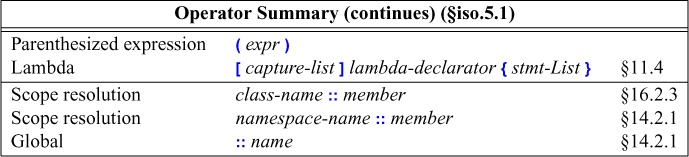
\includegraphics[scale=0.6]{img/017.jpg}
		\caption{Esempio di pianificazione di Nielsen}
		\label{fig: 017}
	\end{center}
\end{figure}

\subsection{Alcuni errori frequenti}
\begin{itemize}
	\item Condurre la valutazione aggregando i problemi e non analizzandoli uno ad uno: \textbf{i problemi di usabilità vanno descritti uno ad uno}
	\item Nella discussione di un problema proporre soluzioni: \textbf{questo lavoro va fatto nella fase DOPO la valutazione euristica, non ne fa parte}
	\item Considerare un principio alla votla e indicare i problemi che violano tale principio: \textbf{in realtà ogni problema può violare più principi, si parte dai problemi}
	\item Mischiare problemi e soluzioni: \textbf{l'output della valutazione è un elenco di problemi prioritizzati}
\end{itemize}

\subsection{Come si prioritizza?}
Per ogni problema identificato dal gruppo, far valutare indipendentemente la severità, e coinvolgere anche una decina di colleghi della azienda e una decina di potenziali utenti (che non siano colleghi dell'azienda).

In poche parole, cercare di ottenere 20-30 valutazioni ordinali di severità per ciascun problema

Il fine è identificare i problemi più urgenti da indirizzare con le risorse a disposizione.

A questo punto si estrae dal sistema di rilevazione (il questionario online) la tabella delle valutazioni (i problemi indicati sulle colonne, le valutazioni di severità nelle righe, una per singolo valutatore).

Per ciascuna riga considerate la classifica di severità adottando la strategia di competizione standard (ovvero un pareggio conta a livello di ordine come due livelli separati, non 1223 ma 1224), costruendo una nuova tabella delle posizioni (a partire da quella delle valutazioni): il o i problemi in testa sono quelli che hanno ottenuto il punteggio più alto.

Considerare 2 fasce: quella dei problemi a priorità più alta considera le prime ne posizioni, con n circa 20\% del numero totale dei problemi, t e poi la fascia delle restanti t-n posizioni. Solitamente nella prima fascia si considerano le prime 3 o 5 posizioni, cioè il podio o una specie di podio allargato. è ragionevole pensare che questi problemi siano responsabili di circa l'80\% di tutti i problemi.

A questo punto contare, per ogni problema, il numero di volte che è in prima fascia (p) e in seconda fascia (s) per ogni utente.

Assegnare il problema definitivamente alla fascia p o s in base al confronto della misura precedente: se p > s allora sarà in p, altrimenti in s.

Eseguire un test binomiale per capire se la differenza tra p ed s è dovuta al caso. In base a questo test si stabiliscono tre fasce in base al P value del test:
\begin{enumerate}
	\item Fascia alta con priorità significativa
	\item Fascia intermedia di non significatività
	\item Fascia bassa con priorità significativa
\end{enumerate}

Nel caso da questo test non sia possibile mettere nessun problema in fascia alta il gruppo può decidere di staccare manualmente dalla fascia intermedia alcuni problemi considerati come di fascia alta.

Tutti i problemi nella fascia di alta priorità significativa dovranno essere risolti prioritariamente e scegliere poi alcuni problemi dalla fascia di non significatività.

Nella tabella dei problemi aggiungere due colonne: in una indicare la fascia di priorità, nell'altra la mediana/media dell'indice di severità indicando anche la deviazione standard.

Per chiarezza, ordinare i problemi mettendo prima quelli che sono in prima fascia e risultati anche significativamente severi. Riportare come nota il numero delle persone coinvolte nella prioritizzazione.

\begin{figure}[h!]
	\begin{center}
		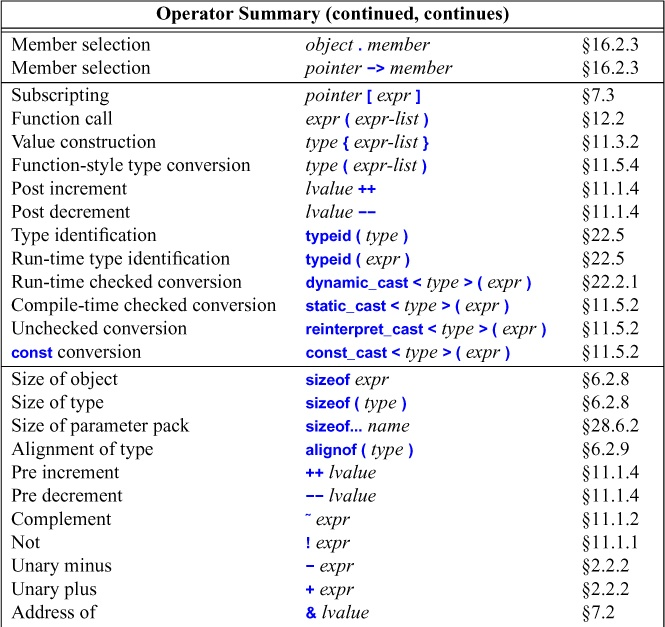
\includegraphics[scale=0.6]{img/018.jpg}
		\caption{Un esempio}
		\label{fig: 018}
	\end{center}
\end{figure}

\subsection{Cosa contiene alla fine la valutazione euristica?}
\begin{itemize}
	\item Descrizione del design sperimentale: cosa avete valutato, perchè, coinvolgendo quante persone, considerando quali task, aerogramma di profilazione, diagramma cartesiano delle expertise...
	\item Elenco finale dei problemi prioritizzati: tabella dei problemi, screenshot dei problemi più gravi, matrice problemi/valutatori, distribuzione problemi/euristiche
	\item Considerazioni finali: legate al numero totale stimato di problemi, alla distribuzione dei problemi, alle citazioni notevoli dalle sessioni olistiche ed esperte
\end{itemize}

L'importante è la prioritizzazione dei problemi di due fasce (priorità più alta, intermedia, più bassa).

Le n schede di analisi da cui è stato redatto l'elenco finale come allegato/appendice.

Meglio uno slideware, non un documento scritto.

Nella cartella di progetto mettere anche le registrazioni e i moduli di consenso.

\section{Statistica inferenziale (approccio quantitativo)}
\subsection{Come potremmo definire il successo di un sistema interattivo?}
\begin{itemize}
	\item gli utenti scelgono il sistema
	\item gli utenti sono disposti a pagare bene per il sistema
	\item la fetta di mercato cresce
	\item il fatturato/ricavi crescono
	\item si viene comprati/copiati da facebook
	\item gli utenti ne parlano bene e lo conosigliano
	\item gli utenti considerano il sistema parte della loro vita
	\item gli utenti preferiscono usare il sistema rispetto altri
\end{itemize}

Ma soprattutto è:
\begin{itemize}
	\item \textbf{Utile}: deve fare quello che viene richiesto
	\item \textbf{Usabile}: deve consentire di fare quello che viene richiesto in modo naturale, senza aumentare i rischi di errore, ecc.
	\item \textbf{Usato}: deve rendere le persone desiderose di usarlo, quindi essere interessante, divertente, piacevole
\end{itemize}

\subsection{Usabilità}
è il grado con cui un prodotto può essere usato da determinati utenti per raggiungere determinati obiettivi con efficacia, efficienza, soddisfazione in un determinato contesto d'uso.

Un altro modo di definirla è il rapporto tra le risorse usate utili per raggiungere il risultato e quelle effettivamente consumate, ovvero la quantità di "spreco" creato.

Notare che differenza può sussistere tra contesti di primo utilizzo, in emergenza, in condizioni di distrazione/affaticamento.

In ogni caso non ha senso parlare di usabilità di un sistema in sè ma in un determinato contesto d'uso. Ha senso parlare di potenziale usabilità.

Possiamo definire delle metriche per misurare il grado di usabilità. Ma qual è la differenza tra metrica e misura?
\begin{itemize}
	\item \textbf{Misura}: risultato della misurazione, assegnazione empirica ed oggettiva di un valore (numerico o simbolo) ad un'entità, per caratterizzarne un attributo specifico
	\item \textbf{Metrica}: comprende la misurazione quantitativa del grado di possesso di uno specifico attributo da parte di un sistema e definisce anche le procedure, modalità e reogole di misurazione. Una metrica stabilisce:
	\begin{itemize}
		\item le entità/attributi da misurare
		\item l'unità di misura
		\item una procedura di misura
	\end{itemize}
\end{itemize}

Quando l'attributo non è fisico e difficilmente misurabile si parla di indicatore, ovvero di proxy tramite il quale leggere un evento.
\begin{figure}[h!]
	\begin{center}
		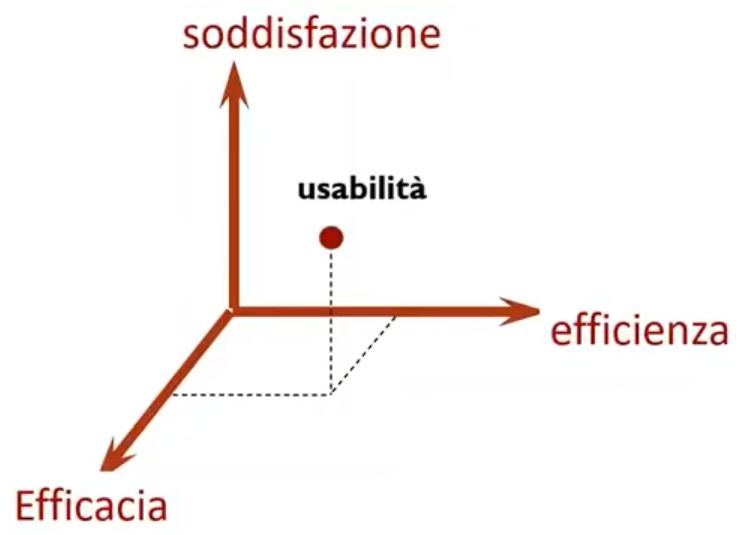
\includegraphics[scale=0.6]{img/020.jpg}
		\caption{Usabilità}
		\label{fig: 020}
	\end{center}
\end{figure}

C'è differenza tra usabilità teorica e usabilità effettiva, questa differenza viene definita come praticamente significativa se e solo se fa effettivamente la differenza, viene invece chiamata statisticamente significativa se non è dovuta al caso.

è possibile avere una differenza statisticamente significativa ma non pragmaticamente (dipende dal contesto) e anche il contrario.

\subsubsection{Usabilità - estensioni}
\begin{itemize}
	\item \textbf{Robustezza}: il sistema deve indurre un basso tasso di errori (o prevenirne proattivamente alcuni), facili da correggere, e con un basso impatto. 
	\item \textbf{Apprendibilità}: facilità nell'apprendere il comportamento del sistema (l'utente lo usa subito per attività utili)
	\item \textbf{Ricordabilità}: facile da ricordare, anche quando un utente riusa il sistema dopo diverso tempo si ricorda come si fa
\end{itemize}

\begin{figure}[h!]
	\begin{center}
		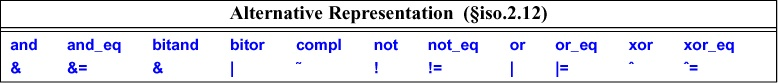
\includegraphics[scale=0.6]{img/021.jpg}
		\caption{Due andamenti tipici di soddisfazione dell'utente nel tempo}
		\label{fig: 021}
	\end{center}
\end{figure}

Ovviamente un sistema che ha entrambi i profili non può esistere ma bisogna sempre trovare un compromesso tra apprendibilità nel breve e alta usabilità (soddisfazione) nel lungo periodo.

\subsubsection{Trade off tra robustezza e efficienza}
Ci può essere un tradeoff tra questi: il desiderio di evitare all'utente errori può portare a progettare un numero eccessivo di vincoli come ad esempio i messaggi di conferma. I trade off devono essere risolti definendo quali dimensioni di usabilità sono più importanti per un certo sistema.

\chapter{Valutazione di qualità/usabilità}
Attività di raccolta dati sull'usabilità di un sistema rispetto a uno specifico gruppo di utenti, nello svolgere una certa attività, in un certo ambiente, o in un certo contesto di lavoro. 

è un'attività:
\begin{itemize}
	\item \textbf{Empirica}: che coinvolge utenti veri
	\item \textbf{Concreta}: eseguita su sistemi reali
	\item \textbf{Sistematica}: da eseguirsi con metodo
\end{itemize}

Si identificano gli obiettivi rilevanti che gli utenti possono raggiungere usando il sistema, quindi i relativi casi d'uso e almeno un percorso/scenawrio principale (happy flow).

Questo è il task su cui valutare il sistema con utenti esperti.

Ci sono due valutazioni:
\begin{itemize}
	\item \textbf{formativa}: aiuta nello sviluppo
	\item \textbf{riassuntiva}: giudizio sul prodotto
	\item[]
	\item \textbf{Assoluta}: misurazione pura
	\item \textbf{Comparativa}: misurazione mettendo a confronto dei valori
	\item[]	
	\item \textbf{Qualitativa}: basata su impressioni soggettive
	\item \textbf{Quantitativa}: basata su test utente e volte a misurare degli attributi di qualità, ad esempio tempi di esecuzione, rapporto tra interazioni corrette ed errori e anche l'opinione degli utenti/esperti quantificata su scale psicometriche
\end{itemize}

Le valutazioni non sono mutualmente escludentisi.

\section{Perchè la valutazione?}
\begin{itemize}
	\item \textbf{Per capire il mondo reale}: come lavora l'utente, come si può migliorare il suo lavoro, la sua attività.
	\item \textbf{Verifica di conformità agli standard}: e.g. la leggibilità dello schermo è accettabile? Gli enti di standardizzazione emettono procedure che permettono di verificare il rispetto degli standard
	\item \textbf{Confrontare progetti/sistemi}: durante l'attività di progetto confrontando prototipi o dopo la realizzazione per capire se il sistema è migliore di altri. Il confronto può essere trasversale o longitudinale
\end{itemize}

\section{Come fare la valutazione di usabilità?}
\begin{itemize}
	\item metodo scientifico:
	\begin{figure}[h!]
		\begin{center}
			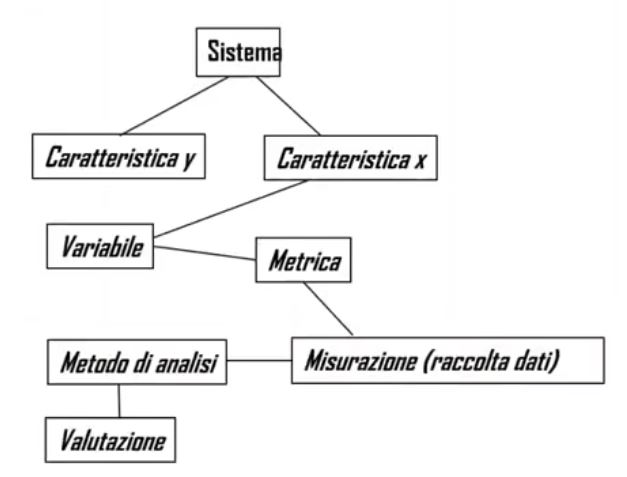
\includegraphics[scale=0.6]{img/022.jpg}
			\caption{Metodo scientifico}
			\label{fig: 022}
		\end{center}
	\end{figure}
	\item metodi sociologici-antropologici (etnografici, etnometodologici, qualitativi):
	\begin{itemize}
		\item Osservazione e monitoraggio: tecniche che derivano dalla sociologia per capire l'interazione nell'ambiente di lavoro
		\item raccolta opinioni degli utenti: metodo strutturati e semi-strutturati per chiedere all'utente cosa pensa e registrare le sue risposte
		\item Interpretativi: dati raccolti con tecniche naturalistiche per non disturbare l'utente e per capire come il sistema si integra con le altre attività.
	\end{itemize}
\end{itemize}

\section{Come si confronta?}
Si raccolgono dati (numerici, ordinali o categorici) da un campione di utenti del sistema.
\begin{itemize}
	\item Variaibli scalari (numeriche): sono valori assoluti
	\item Variabili ordinali: in cui è possibile stabilire un ordine totale sui possibili valori/attributi
	\item Variabili categoriche o nominali: in cui i valori sono modalità, ovvero parole
\end{itemize}

\begin{figure}[h!]
	\begin{center}
		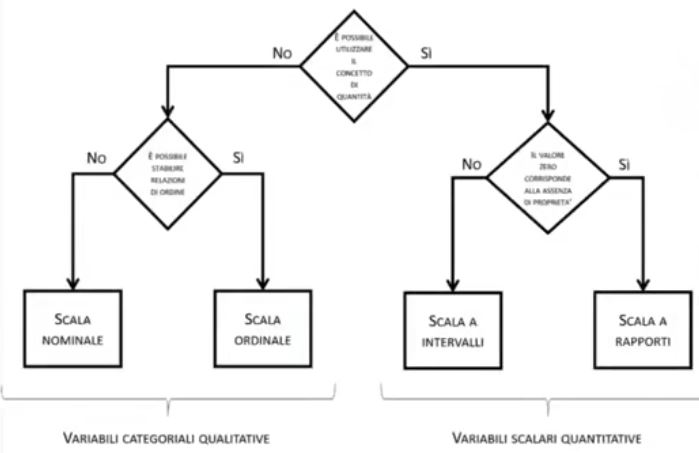
\includegraphics[scale=0.6]{img/023.jpg}
		\caption{Tipi di variabile}
		\label{fig: 023}
	\end{center}
	\begin{center}
		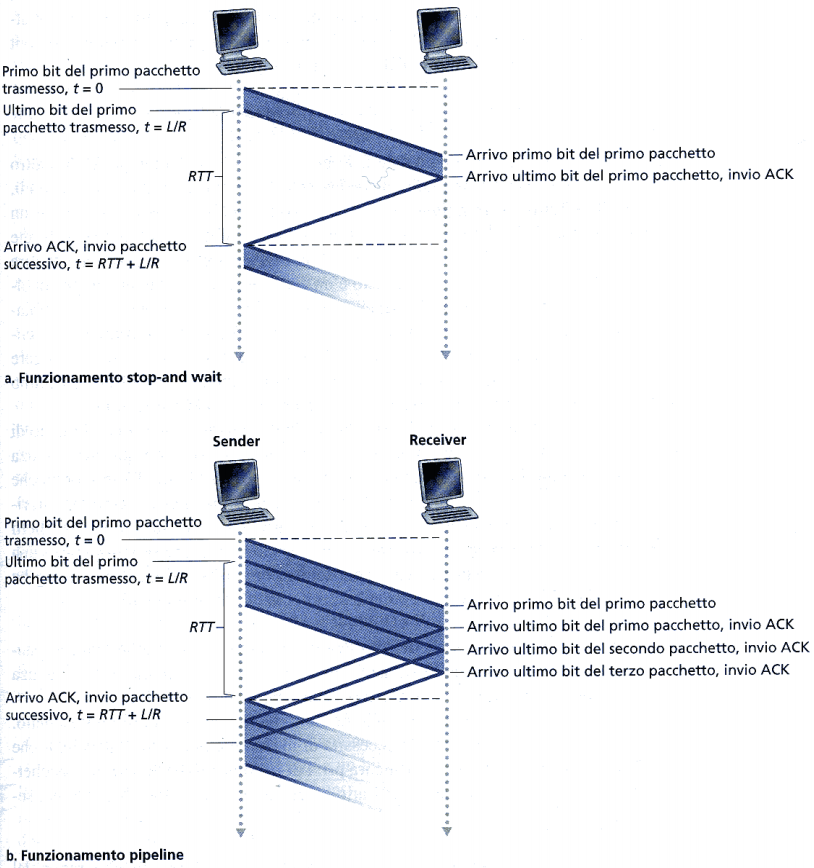
\includegraphics[scale=0.6]{img/024.jpg}
		\caption{Cosa fare in base al dato}
		\label{fig: 024}
	\end{center}	
\end{figure}

\subsection{Procedura}
\begin{enumerate}
	\item Si raccolgono dati da un campione di utenti del sistema
	\item si calcolano le statistiche
\end{enumerate}

Non potendo conoscere il parametro della popolazione ma solo la statistica di un campione non si può essere precisi, ci sarà sempre un errore standard, ma per si può stimare l'intervallo che è ragionevole pensare contenga il parametro "vero", questo è l'intervallo di confidenza. RIcordare che l'intervallo di confidenza è l'intervallo di valori che si è abbastanza confidenti che contenga il valore vero del parametro. Indica l'incertezza intrinseca della stima.

\begin{figure}[h!]
	\begin{center}
		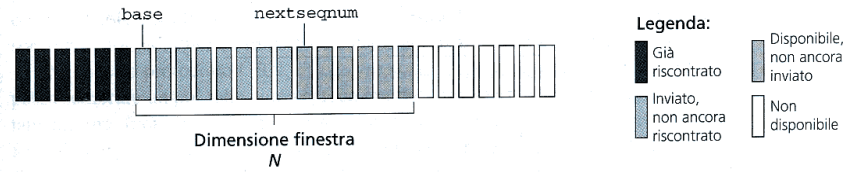
\includegraphics[scale=0.6]{img/025.jpg}
		\caption{Errore standard}
		\label{fig: 025}
	\end{center}
\end{figure}

Per la media $ES=\dfrac{\sigma}{\sqrt{N}}$, per le proporzioni $ES=\sqrt{\dfrac{(p*(1-p))}{N}}$
Strumenti utili:
\begin{itemize}
	\item \href{http://vassarstats.net/conf_mean.html}{Calcolo confidenza per le medie}
	\item \href{http://vassarstats.net/prop1.html}{Calcolo confidenza per le proporzioni}
\end{itemize}

\subsubsection{Approccio di Neyman}
Si confrontano gli intervalli di confidenza.
\begin{figure}[h!]
	\begin{center}
		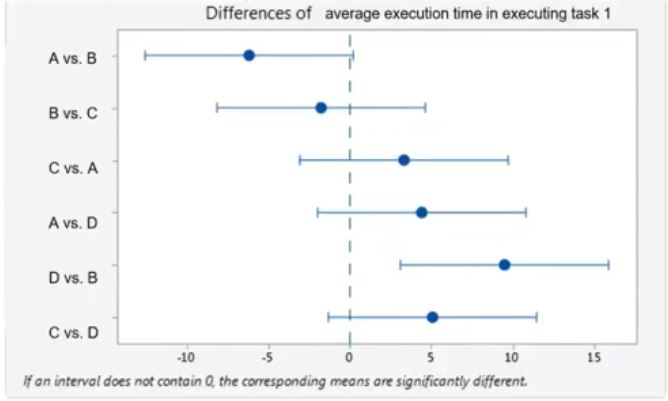
\includegraphics[scale=0.6]{img/026.jpg}
		\caption{Differenze di tempo di esecuzione media di un task}
		\label{fig: 026}
	\end{center}
	\begin{center}
		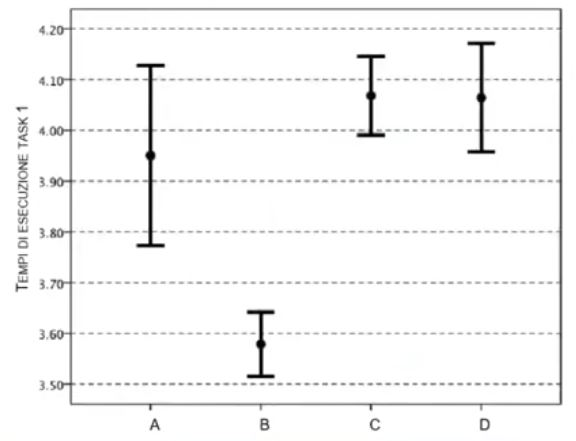
\includegraphics[scale=0.6]{img/027.jpg}
		\caption{Intervalli di confidenza dei singoli valori}
		\label{fig: 027}
	\end{center}
\end{figure}
Tra questi sistemi solo D vs B differiscono per i tempi di esecuzione del task 1 in quanto è l'unico confronto in cui la differenza 0 non è inclusa nell'intervallo di confidenza. Lo si può notare anche dalla visualizzazione degli intervalli di confidenza dei singoli valori e non della loro media. Se i due intervalli di confidenza non si sovrappongono sulle ordinate allora c'è una differenza significativa.

\subsubsection{Approccio di Fisher}
Si formulano test di ipotesi e si verificano con essi le ipotesi null ($H_0$).

L'ipotesi nulla è assunta vera e prevede che non ci sia differenza tra:
\begin{itemize}
	\item i sistemi $s_1$ e $s_2$ (per la medesima caratteristica), o
	\item per il sistema s tra la versione a tempo $t_0$ e quella a $t_1$, o
	\item tra strati (gruppi) di utenti (ad esempio, maschi vs femmine, giovani vs senior, esperti vs non esperti)
\end{itemize}

Se non si riesce a rigettare l'ipotesi nulla non significa che questa sia vera.

\subsubsection{The null ritual (O null hypothesis testing)}
Un incrocio tra l'approccio di Neyman e di Fisher.
\begin{enumerate}
	\item Si sceglie il test giusto per l'ipotesi e il tipo di dato che si raccoglie (vedere l'immmagine a pagina \pageref{fig: 024})
	\item si esegue il test e si calcola il corrispondente "livello di significatività osservato" dei dati (p value)
	\item si riportano i risultati in uno stile chiaro e "confrontabile" (e.g. standard APA)
\end{enumerate}

\begin{figure}[h!]
	\begin{center}
		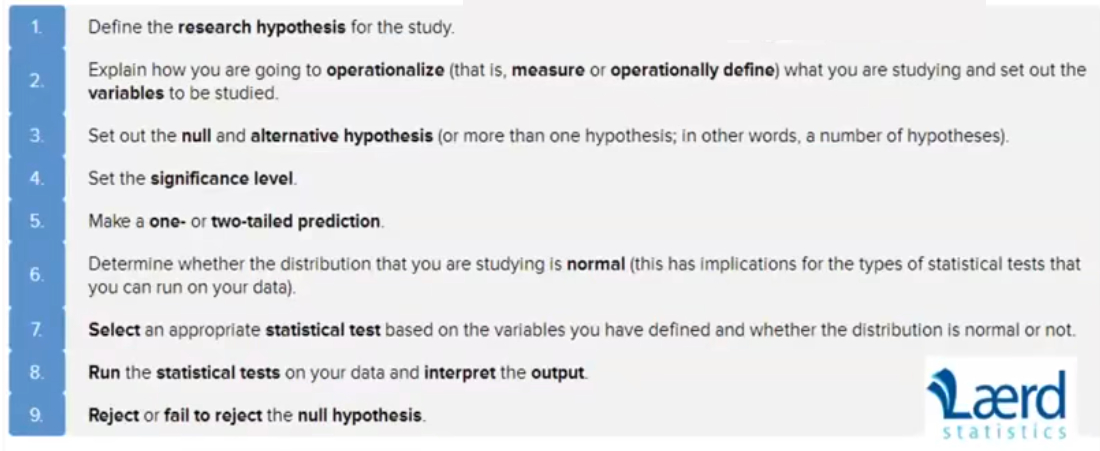
\includegraphics[scale=0.6]{img/028.jpg}
		\caption{Lista dei passi}
		\label{fig: 028}
	\end{center}
\end{figure}
\paragraph{Passo 3}
Il livello di significatività del test (o alpha) solitamente è posto al 5\% all'1\%. Alpha è la probabilità associata al rischio che siamo disposti a correre di rigettare l'ipotesi nulla quando questa è vera (cioè di prendere un falso positivo, o errore del I tipo). Gli errori più gravi sono quelli di II tipo.
\begin{figure}[h!]
	\begin{center}
		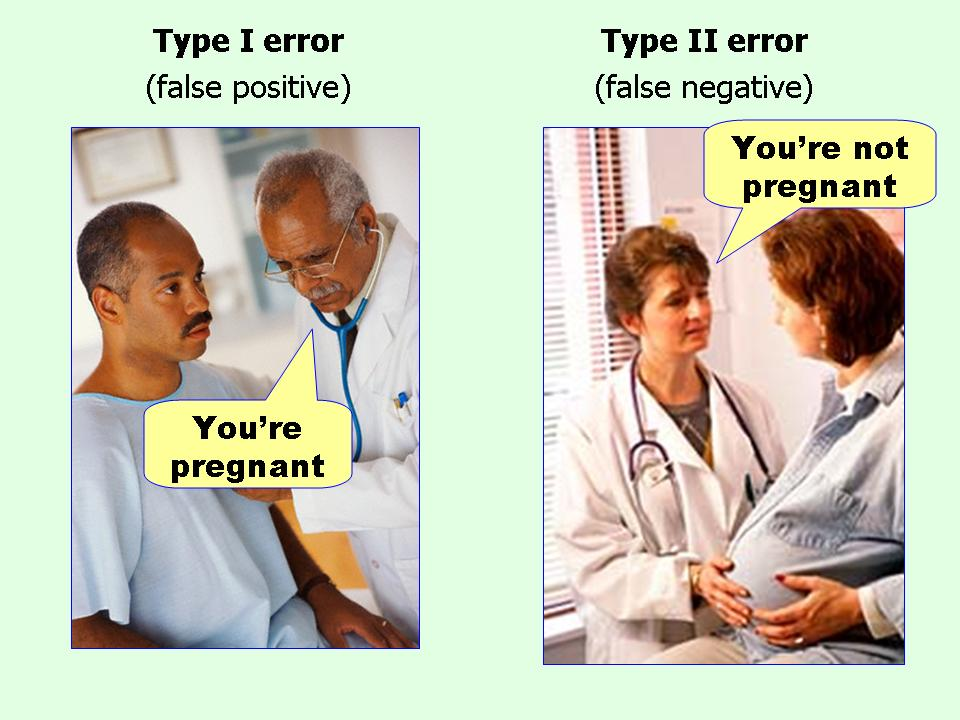
\includegraphics[scale=0.6]{img/029.jpg}
		\caption{Errori di I e II tipo}
		\label{fig: 029}
	\end{center}
\end{figure}

Un test è più potente in base a quanto è abile di rilevare il caso nel quale si rigetta l'ipotesi nulla. Solitamente, in ambito accademico, si usa l'euristica di Cohen: Alpha 4 volte più piccolo di Beta (e.g. $\alpha=.05, \beta=.20$). In ambito industriale si usa una Beta più piccola. La specificità è $1-\alpha$, la sensitività è $1-\beta$. La specificità è la capacità del test di evitare i falsi positivi, la sensitività è la capacità di evitare falsi negativi.

\paragraph{Passo 4}
Due code per predire differenza in un verso o nell'altro (A è meglio o peggio di B), una coda per differenza in un verso preciso (A è meglio di B, non peggio).

\paragraph{Passi 7 e 8}
\begin{figure}[h!]
	\begin{center}
		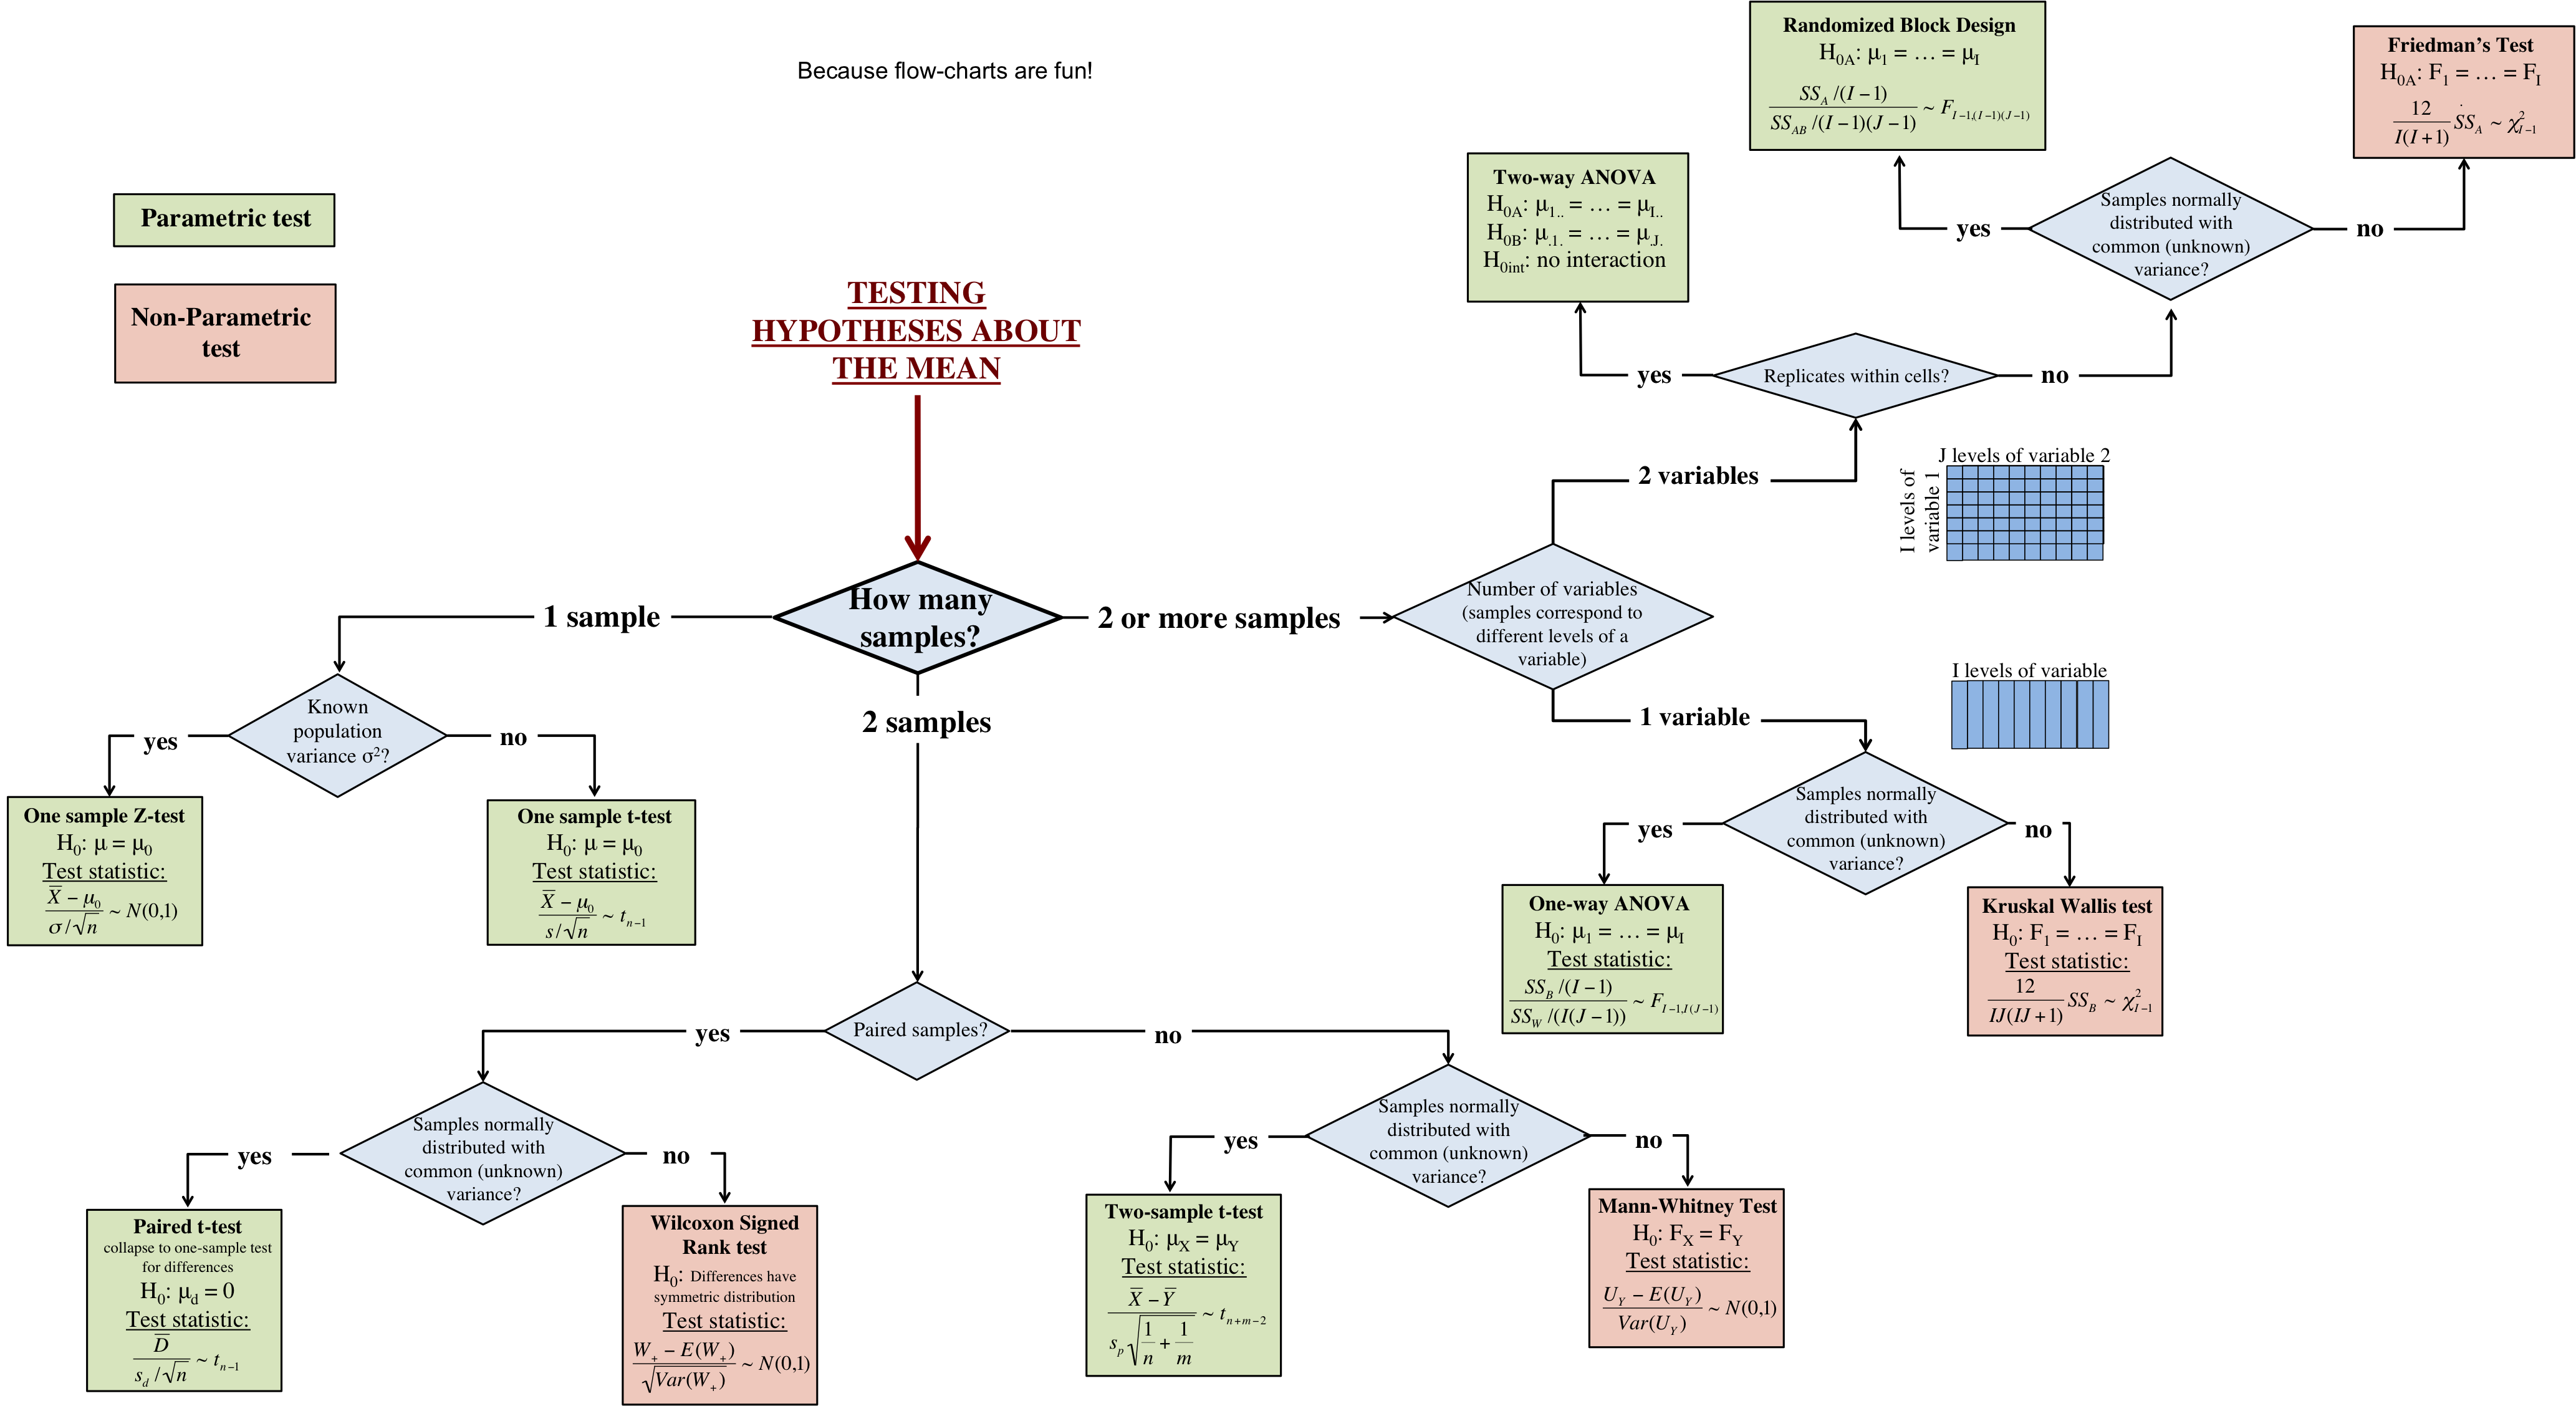
\includegraphics[scale=0.1]{img/030.png}
		\caption{Testare le ipotesi riguardo la media}
		\label{fig: 030}
	\end{center}
\end{figure}

Ricordiamo: il p-value è la probabilità di raccogliere dati come quelli raccolti (o ancora più estremi) assumendo l'ipotesi nulla $H_0$ come vera,



\chapter{Lessico} 
\paragraph{Ergonomia}
Disciplina scientifica che si occupa dei problemi relativi al lavoro umano in rapporto alla progettazione delle macchine e agli ambienti di lavoro, al fine di individuare le soluzioni più idonee alle esigenze psicofisiche dei lavoratori e al contempo a quelle della produzione.

\paragraph{Sistema socio tecnico}
Pagina \pageref{par: sistema sociotecnico}.

\begin{itemize}
	\item è un sistema, "un insieme di elementi interrelati ed eventualmente mutuamente dipendenti che, agli occhi di un osservatore esterno, appaiono come un'entità unitaria ma collettiva, con caratteristiche e comportamento proprio, solitamente autonomo ed intenzionale (cioè volto ad un obiettivo)";
	\item Un sistema in cui la componente umana  (sociale) e quella tecnica (tecnologica) sono inestricabilmente legate tra loro e la loro interazione porta a fenomeni emergenti impredicibili. Attenzione che tecnica è un termine generico proprio per intendere tutti gli strumenti, che siano fisici o dell'ingegno. In più si parla di interdipendenza perchè lo strumento è fermo senza qualcuno che lo usa, l'umano è fermo se non ha uno strumento per agire;
	\item è un concetto di invarianza di scala, ovvero il concetto non cambia in base alla grandezza dell'ambiente sociale
\end{itemize}

\paragraph{Affordance}
Pagina \pageref{par: affordance}.

Gibson: è la risorsa o supporto che l'ambiente offre all'utente

Norman: è una qualsiasi proprietà o qualità di un oggetto che definisce i suoi possibili utilizzi o rende chiaro come possa o debba essere usato.

Una affordance è qualsiasi proprietà di un oggetto che invita una persona competente all'azione mediata da tale oggetto.

\paragraph{Mapping}
Pagina \pageref{par: mapping}.

É il rapporto fra i comandi, il loro azionamento ed i risultati che ne derivano nel mondo esterno; permette all’utente di creare un collegamento diretto fra i comandi di controllo e le parti dell’oggetto di cui modificano rispettivamente lo stato.
\paragraph{Porte di Norman}
Pagina \pageref{par: porta di norman}.

Una porta di Norman è una porta il cui design suggerisce un'azione contraria a quella da fare o che richiede un segnale per spiegare come usarla.

\paragraph{Toilette di Floyd}
Pagina \pageref{par: toilette di Floyd}.

Una toilette di floyd è un qualcosa di progettato in maniera così poco intuitiva per il quale devo fornire una serie di istruzioni.

\paragraph{Sistema interattivo e interfaccia}
Pagina \pageref{par: sistema interattivo}.

Per interfaccia d'uso (o interfaccia utente, user interface) intendiamo l'insieme di “tutti i componenti di un sistema interattivo (software o hardware) che forniscono all'utente informazioni e comandi per permettergli di effettuare specifici compiti attraverso il sistema.

\paragraph{Automation bias/overreliance}
Pagina \pageref{par: automation bias}.

è l'eccessiva fiducia nella risposta del supporto alle decisioni e quindi causa di errori di omissione o di azione quando i sistemi sono imperfetti (e.g. la calcolatrice che deve rispondere correttamente, non può essere altrimenti). è legato ai processi decisionali.

\paragraph{Errori di giustapposizione}
Quando a causa della posizione specifica di un elemento si preme un pulsante differente rispetto a quello desiderato (e.g. due elementi in un menù a tendina che sono molto vicini tra loro)

\paragraph{Workaround}
Pagina \pageref{par: workaround}.

Qualsiasi azione relativa all'esecuzione di un processo o di un compito (supportati dal sistema informatico) che non è prevista o descritta nei manuali di uso del sistema informatico e/o nei manuali che descrivono tale processo o procedura e che può bypassare l'uso del sistema o piegarlo ai propri fini.

\paragraph{Complessità strutturale, funzionale e d'uso}
Pagina \pageref{par: complessità}.

\begin{itemize}
	\item \textbf{Complessità funzionale}: indica quante funzioni possono essere svolte tramite l'interfaccia in analisi (un cacciavite a punta singola ha una bassa complessità funzionale, un coltellino svizzero ha un'alta complessità funzionale in quanto in base a come viene usato può svolgere numerose funzioni in virtù delle sue componenti)
	\item \textbf{Complessità strutturale}: indica, genericamente, quanto sia complessa la struttura di uno strumento (un cucchiaio ha una complessità strutturale bassa, uno smartphone una complessità strutturale alta)
	\item \textbf{Complessità d'uso}: indica quando sia semplice utilizzare l'interfaccia, ha un forte elemento basato anche sulle capacità personali (una maniglia ha complessità d'uso bassa, una macchina con cambio manuale ha complessità d'uso alta)
\end{itemize}

\paragraph{Euristica e valutazione euristica}
Pagina \pageref{par: euristica}.

Una euristica è un insieme di concetti, riferimenti e, soprattutto, strategie che si sono rilevate particolarmente adatte a risolvere un determinato problema, nel nostro caso la progettazione di sistemi interattivi usabili.

La valutazione euristica è la valutazione (di usabilità) svolta alla luce di un determinato insieme di euristiche (ben definite, possibilmente ben note, prese a riferimento) per identificare soluzioni di design che o si conformano o violano una o più euristiche di tale insieme.

\paragraph{Segno, simbolo, indice, icona}


\paragraph{Significante, significato, oggetto}


\paragraph{Metacomunicazione}


\paragraph{Deputy del progettista}
L'oggetto creato rappresenta l'artista che lo crea.

\paragraph{Captologia}


\paragraph{Soggettivismo - oggettivismo}


\section{"Metodologia"}
\begin{figure}[h!]
	\begin{center}
		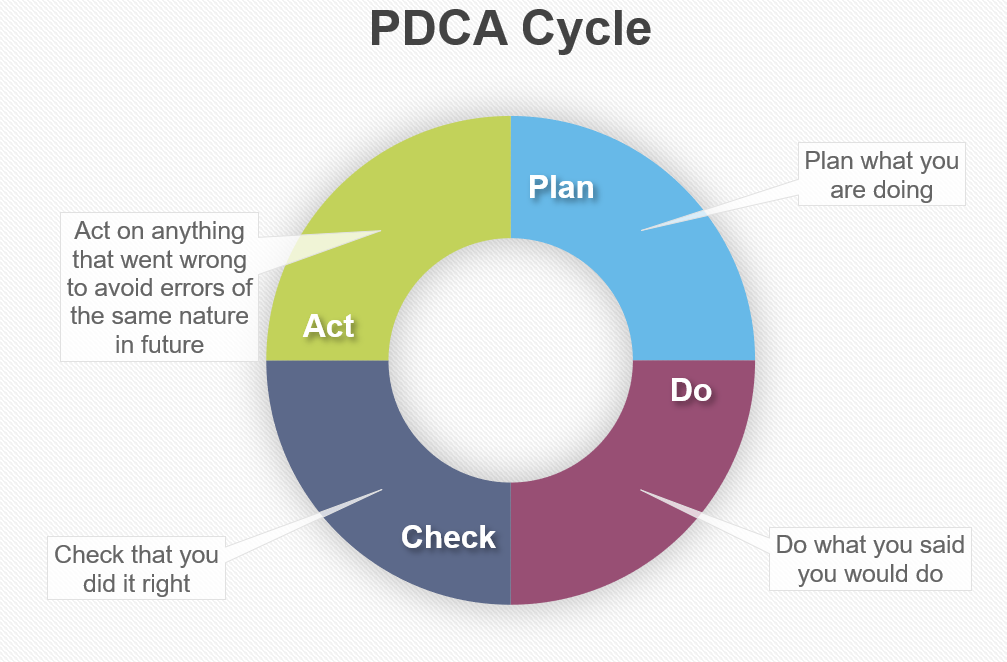
\includegraphics[scale=0.4]{img/011.png}
		\caption{PDCA cycle}
		\label{fig: 011}
	\end{center}
\end{figure}
\begin{itemize}
	\item Affina sensibilità per il brutto e il cattivo
	\item Progetta in equilibrio tra familiarità e originalità
	\item Sappi che parli all'utente anche di te stesso
	\item Non guardarti l'ombelico ma coinvolgi gli utenti
	\item Trova i problemi, prioritizzali e risolvili
	\item Valuta usabilità in termini di efficienza, efficacia e soddisfazione
	\item Migliora il tuo artefatto
	\item Torna agli utenti
\end{itemize}

\paragraph{Usabilità}
è il grado con cui un prodotto può essere usato da determinati utenti per raggiungere determinati obiettivi con efficacia, efficienza, soddisfazione in un determinato contesto d'uso.

\paragraph{P-value}
La probabilità di raccogliere dati come quelli raccolti (o ancora più estremi) assumendo l'ipotesi nulla $H_0$ come vera,
\end{document}
